% SPDX-FileCopyrightText: 2023 SAP SE
%
% SPDX-License-Identifier: Apache-2.0
%
% This file is part of FEDEM - https://openfedem.org

%%%%%%%%%%%%%%%%%%%%%%%%%%%%%%%%%%%%%%%%%%%%%%%%%%%%%%%%%%%%%%%%%%%%%%%%%%%%%%%%
%
% FEDEM User Guide.
%
%%%%%%%%%%%%%%%%%%%%%%%%%%%%%%%%%%%%%%%%%%%%%%%%%%%%%%%%%%%%%%%%%%%%%%%%%%%%%%%%

\def\Variable#1{\textless#1\textgreater}
\def\Untitled{\File{untitled\_\Variable{\#}.fmm}}


\Chapter{Learning the Basics}{learning-the-basics}

This chapter outlines some system requirements,
explains how and where models and their results are saved,
and introduces the Fedem GUI with some basic commands.

Sections in this chapter address the following topics:

\begin{itemize}
\item
  \protect\hyperlink{system-requirements}
                    {System requirements}
\item
  \protect\hyperlink{storing-models-and-results}
                    {Storing models and results}
\item
  \protect\hyperlink{starting-fedem}
                    {Starting Fedem}
\item
  \protect\hyperlink{touring-the-interface}
                    {Touring the interface}
\item
  \protect\hyperlink{executing-commands}
                    {Executing commands}
\item
  \protect\hyperlink{visualizing-the-model}
                    {Visualizing the model}
\item
  \protect\hyperlink{opening-and-saving-model-files}
                    {Opening and saving model files}
\item
  \protect\hyperlink{loading-and-unloading-fe-data}
                    {Loading and unloading FE-Data}
\item
  \protect\hyperlink{exporting-objects}
                    {Exporting objects}
\item
  \protect\hyperlink{customizing-fedem-using-plug-ins}
                    {Customizing Fedem using plug-ins}
\item
  \protect\hyperlink{customizing-fedem-using-addons}
                    {Customizing Fedem using Addons}
\end{itemize}

\clearpage


%%%%%%%%%%%%%%%%%%%%%%%%%%%%%%%%%%%%%%%%%%%%%%%%%%%%%%%%%%%%%%%%%%%%%%%%%%%%%%%%
\Section{System requirements}{system-requirements}

The following are minimum system/hardware requirements and recommended
settings for optimal Fedem performance.

\Note{Use of resolution settings other than those recommended below may
  require you to move or resize windows and dialog boxes to fit your screen.}

\begin{center}
\begin{threeparttable}[b]
\begin{tabular}{ | m{3.5cm} | m{6.5cm} | }
    \hline
    \textbf{Processor}  & Recommended: Pentium 4 @ 2 GHz. \newline
                          Minimum: Pentium III @ 850 MHz. \\ \hline
    \textbf{RAM}  & Recommended: 2 GB. Minimum: 256 MB. \\ \hline
    \textbf{Free disk space} &  Dependent upon the size and complexity of mechanism models.\tnote{1} \\ \hline
    \textbf{Graphics card}   & Recommended: high end graphics card. \newline
                     Required: OpenGL\Registered API support. \\ \hline
    \textbf{Pointing device} &  Three-button mouse with wheel. \\ \hline
    \textbf{Resolution setting} &  1,280 x 1,024 pixels or higher. \\ \hline
\end{tabular}
\begin{tablenotes}
  \item[1]{Larger models may require several GBs.}
\end{tablenotes}
\end{threeparttable}
\end{center}


%%%%%%%%%%%%%%%%%%%%%%%%%%%%%%%%%%%%%%%%%%%%%%%%%%%%%%%%%%%%%%%%%%%%%%%%%%%%%%%%
\Section{Storing models and results}{storing-models-and-results}

Fedem uses the following files and directories to store the contents of a model:

\begin{itemize}
\item The mechanism assembly description and all simulation parameters
  are saved in the Fedem Mechanism Model (\File{.fmm}) format.
  This file is called the model file and contains the complete description
  of your model except for the FE data files and the simulation results.
\item FE data files and all simulation results are saved in a directory named
  \File{\Variable{modelfilename}\_RDB} (the model name specified by the user
  is substituted for \File{\Variable{modelfilename}}).
  Fedem creates this directory in the same location as your model file.
  Within this directory, the FE data files are stored in a directory named
  \File{link\_DB}, unless a FE model repository is used
  (see \refSection{using-fe-model-repositories}{Using FE model repositories}).
\end{itemize}

\refAppendix{file-types-and-usage}{File Types and Usage} contains more
information about Fedem file types, whereas the directory structure is shown in
\refSection{rdb-directory-structure}{RDB directory structure}.


\SubSection{FTL format}{ftl-format}

The Fedem Technology Link (\File{.ftl}) format is used to store
FE models as sets of data in text format
(see \refSection{fedem-technology-link-format}{Fedem Technology Link format}
for more information about the \File{.ftl} file format).


\SubSection{FTC format}{ftc-format}

The Fedem Technology Cad (\File{.ftc}) format may be used to store CAD
geometry in text format.


\SubSection{Other supported formats}{other-supported-formats}

Fedem can import FE models
(see \refSection{creating-parts-by-file-import}{Creating parts by file import})
in the MSC.Nastran Bulk Data File (\File{.bdf} or \File{.nas}) format
(see \refSection{nastran-bulk-data-file-format}{Nastran Bulk Data File format})
and the SESAM input interface file (\File{.FEM}) format.
Earlier versions used the Fedem Link Model (\File{.flm}) format.
This file format is still supported for backward compatibility.

Fedem can also import CAD geometry from VRML files (\File{.wrl}, \File{.vrml},
\File{.vrl}, \File{.wrz}) for visualization of Generic Parts
(see \refSection{parts}{Parts}).


%%%%%%%%%%%%%%%%%%%%%%%%%%%%%%%%%%%%%%%%%%%%%%%%%%%%%%%%%%%%%%%%%%%%%%%%%%%%%%%%
\Section{Starting Fedem}{starting-fedem}

Fedem can be started from either the Windows Start menu,
the Windows file browser, or the command prompt.

\begin{itemize}
\item To start Fedem with a new, empty model, press the Fedem icon on the
  Windows Desktop or choose \textbf{Fedem} from the Windows Start menu.
\item To start Fedem and open an existing model, double-click the icon
  representing the desired model file in the Windows file explorer.
\item Open a command prompt, navigate to the installation directory of Fedem
  and type \File{fedem} optionally followed by some command line options
  (see \refSection{command-line-options}{Command-line options}).
\item To open an existing model from the command prompt,
  navigate to the installation directory and type
  \File{fedem -f \Variable{modelpath}.fmm} substituting
  \File{\Variable{modelpath}} with the path and base name of your model file.
  Alternatively, navigate to the directory of the model file and type
  \File{\Variable{installationdir}/fedem -f \Variable{modelfile}.fmm}, where
  \File{\Variable{installationdir}} is replaced by
  the directory name of the Fedem installation, and
  \File{\Variable{modelfile}} is the base name of the model.
\end{itemize}

When Fedem is started with a new, empty model, the model file is named
\Untitled, where \File{\Variable{\#}} indicates a unique running number. This
empty model file will contain only some default settings, animations and graphs.
The file will be created in your default login directory when Fedem is started
from the Desktop icon or from the Windows Start menu.


\SubSection{Command-line options}{command-line-options}

Fedem has several command-line options that can be used to achieve
different tasks or settings. These options can be invoked when starting
Fedem from the command prompt. Among others, you have options for
starting Fedem in batch mode without any GUI at all, which is useful when
you just want to run an existing model without modifying it.
Refer to \refSection{fedem-gui-options}{Fedem GUI options}
for the complete list of available command-line options.

\Tip{You can create a new model file with a specific name by specifying
  a path and filename that does not yet exist, using the -f option.
  The file will be created for you and opened when Fedem starts.}


\SubSection{Template model file}{template-model-file}

The default settings of a new model are stored in a template model file
which is loaded whenever a new model is created
(either when Fedem is started, or when using the \textbf{New} command,
see \refSection{starting-a-new-model}{Starting a new model"}).
The template file can be modified or changed as needed, and is located in
\File{\Variable{installationdir}/Templates/default.fmm}.

If a different location for the template file is wanted, the environment
variable FEDEM\_TEMPLATE\_FILE can be defined to contain the desired
path to the template file.

\subsubsection{Predefined template files}

The \File{Templates} directory of the Fedem installation contains three
files; \File{default.fmm}, \File{default\_m.fmm} and \File{default\_mm.fmm}.
The files \File{default.fmm} and \File{default\_m.fmm} are identical and
suitable for models using SI unit set, while \File{default\_mm.fmm} contains
default settings that are suitable for models using millimeter, newton and
mega gram as unit set. Simply copy the file \File{default\_mm.fmm} to
\File{default.fmm} if you prefer mm/N/Mg as your default unit set.


\SubSection{Console window}{console-window}

When Fedem is started on a Windows system, a separate console window can
be opened in addition to the Fedem main window, by specifying the
command-line option \File{-console}. This window lists some startup
messages, and may also contain some low-level error messages during a
Fedem session, that normally can be ignored by users, but sometimes
might help understanding an abnormal incident.

\Warning{Once opened, the separate console window must remain open
  throughout the whole Fedem session; closing it explicitly closes the entire
  Fedem session immediately, without the option to save unsaved work.}

\Tip{If abnormal behavior occurs, or if Fedem stops responding,
  check the console window (if activated) and the Output List
  (discussed later) for important information.
  Take note of any errors or warnings before contacting Fedem technical support
  (\href{mailto:support@fedem.com}{\nolinkurl{support@fedem.com}}).}

After finishing some initial setup tasks, the Fedem GUI main window will appear.
In the following sections, the Fedem GUI is described in detail.


%%%%%%%%%%%%%%%%%%%%%%%%%%%%%%%%%%%%%%%%%%%%%%%%%%%%%%%%%%%%%%%%%%%%%%%%%%%%%%%%
\Section{Touring the interface}{touring-the-interface}

\SubSection{Main window}{main-window}

Starting with an empty model file,
the main window of the Fedem GUI appears, as shown below.

\begin{figure}[H]
  \begin{picture}(360,260)
    \put(-80,169){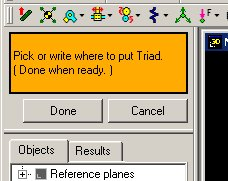
\includegraphics[width=0.2\textwidth]{Figures/2-Guide}}
    \put(15,0){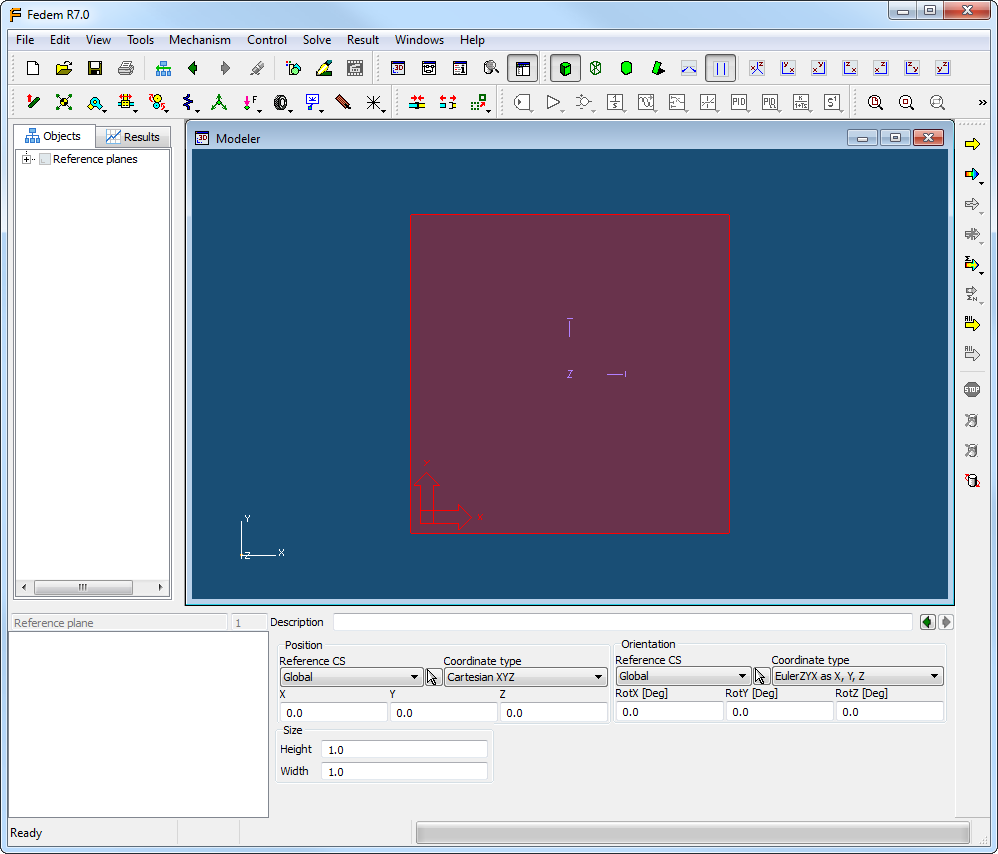
\includegraphics[width=0.85\textwidth]{Figures/2-MainUI}}
    \put(-8,222){\Bullet{1}\huge\{}
    \put(55,205){\Bullet{2}}
    \put(-88,215){\Bullet{3}}
    \put(100,205){\Bullet{4}}
    \put(55,53){\Bullet{5}}
    \put(120,55){\Bullet{6}}
    \put(40,1){\Bullet{7}}
  \end{picture}
\end{figure}

\begin{bulletlist}
\item{\sl Menus and tool bars} --
  contain buttons used to initiate commands.
\item{\sl Model Manager panel} --
  contains the {\sl Objects} and {\sl Results} tabs, which allow you to create,
  manage, and delete the objects in your model and define Animations and Graphs
  of your results.
\item{\sl Guide panel} --
  This orange panel may pop up above the Model Manager panel when you invoke
  a command. It will tell you what you are expected to do during the different
  steps of the command. It also provides \textbf{Done} and \textbf{Cancel}
  buttons used to accept choices or to cancel the command, respectively.
\item{\sl Workspace area} --
  contains the {\sl Modeler}, {\sl Control Editor} and {\sl Graph} views
  for constructing and viewing models and results.
\item{\sl ID and Topology panel} --
  lists objects related to the selected item.
\item{\sl Property Editor panel} --
  allows you to view and edit the properties of individual objects in the model.
\item{\sl Status bar} --
  provides information of the status, progress information
  and whether a solver process is running.
\end{bulletlist}


\SubSection{Menus and tool bars}{menus-and-tool-bars}

Fedem commands are initiated from buttons on the tool bars and menus.
All commands can be accessed from the menus, while the tool bars display only
the most commonly used commands.
The menus are arranged from left to right in logical order of task execution,
starting with standard file functions, then continuing with viewing commands,
mechanism modeling, control system modeling, analysis/solution tools,
and finally results management.


\subsubsection{Command sensitivity}

Menu and tool bar buttons are sensitive to the active view and object
selection. For example, if an object in the {\sl Modeler} view is
selected, the {\sl Graph} view controls appear dimmed (grayed-out) and
cannot be selected.

\subsubsection{Fedem tool bars}

Fedem uses the following tool bars (a tool bar handle to the left (or on
top) marks the beginning of a tool bar):

\begin{itemize}
\item{\sl Standard} --
  provides standard file operations such as \textbf{Open}, \textbf{Save},
  \textbf{Exit}, and selecting and deleting objects.
\item{\sl Windows} --
  provides commands for controlling the active view selection
  ({\sl Modeler}, {\sl Control Editor}, {\sl Output List},
  {\sl Result File Browser})
  and hiding/showing the Model Manager and Property Editor panels.
\item{\sl Zoom and Pan} --
  provides commands for zooming and panning of {\sl Graph} view displays.
  (See \refSection{zoom-and-pan}{Zoom and Pan} for more information
  about these commands.)
\item{\sl 3D View Control} --
  includes commands for rotating the view and changing the view perspective
  in the {\sl Modeler} view. (See \refSection{view-controls}{3D View controls}
  for information about manipulating the view.)
\item{\sl Solvers} --
  these commands are used to set up, start, and stop mechanism analyses,
  and to calculate specific results.
  (See \refChapter{mechanism-analysis}{Mechanism Analysis} for information
  about these commands.)
\item{\sl Mechanism Creation} --
  contains commands for importing parts and creating mechanism entities
  such as Joints, Springs, Dampers, Forces, Sensors, etc.
  (See \refChapter{mechanism-elements}{Mechanism Elements} for more information.)
\item{\sl Mechanism Tools} --
  provides commands used in modeling such as moving, attaching, copying objects,
  and applying motion constraints.
  (See \refChapter{mechanism-elements}{Mechanism Elements}
  for information about modeling tools.)
\item{\sl Control Creation} --
  provides commands for creating control objects.
  (See \refChapter{control-system-modeling}{Control System Modeling}
  for detailed descriptions of control objects.)
\item{\sl Control Tools} --
  contains commands for manipulating the control system.
  (See \refChapter{control-system-modeling}{Control System Modeling}
  for information about modeling control systems.)
\end{itemize}

\SubSubSection{Manipulating tool bars}{manipulating-tool-bars}

\begin{wrapfigure}{r}{0.25\textwidth}
  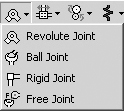
\includegraphics[width=0.25\textwidth]{Figures/1st_Joint_Pulldown}
\end{wrapfigure}

Only some of the commands accessible from the tool bars are displayed. You will
see that there are arrows ($\blacktriangledown$) beside some of the icons.
To access other commands, click and hold down the $\blacktriangledown$ button.
A menu of additional, related commands is displayed (example at right).
Selecting a command from the menu initiates the command and replaces the
button’s function with that of the new command. You can select another
option at any time by clicking, holding down the $\blacktriangledown$ button,
and selecting a different command.

\clearpage
Fedem provides several ways to manage tool bars:

\begin{itemize}
\item Right-click a tool bar handle and select an option
  to relocate, show, or hide the tool bar.
\item Right-click an empty space in the tool bar area and select
  an option from the list to show or hide a tool bar.
\item Double-click a tool bar handle to show or hide the tool bar.
\item Drag a tool bar handle to the left, right, top, or bottom of
  the main window to relocate the tool bar.
\end{itemize}


\SubSection{Model Manager}{model-manager}

\begin{wrapfigure}{r}{0.35\textwidth}
  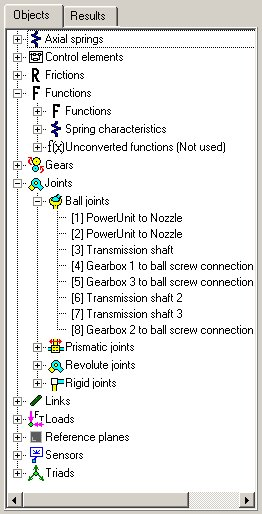
\includegraphics[width=0.35\textwidth]{Figures/2-ModelManager}
\end{wrapfigure}

The Model Manager Panel contains lists of all the objects and result views
that make up your model. This includes mechanism, modeling, and control
system objects, along with animations and graphs. In each list,
objects are grouped by type and sorted by identification numbers or names.
In the Model Manager panel, right-click menus can access several
commands that can be applied to the selected objects.

% Can't use the \Note macro here due to the wrapfigure above
\MiniGenericNote{note}{NOTE}{-25mm}{0.8}{0.13}{0.7}{
  The Objects and Results lists are empty (or nearly empty)
  until you create some items.}

\SubSubSection{Selecting items}{selecting-items}

In the Model Manager panel, you can select items in several ways:
\begin{itemize}
\item Highlight a single item.
\item Hold down the Shift key and click multiple items.
\item Hold down the Ctrl key and click multiple items
  (or a single item to select/deselect).
\item Click and drag the mouse over multiple items.
\end{itemize}

\subsubsection{Deselecting items}

To deselect all items, right-click an empty space in the Model Manager panel.

\subsubsection{Sorting}

The objects in the Model Manager panel can be sorted, either by ID-number or
by item name. To switch sorting mode, right-click inside the panel and
select either Sort by ID or Sort by Name from the menu that appears.
By default, the sorting is based on ID-numbers.

\Tip{Right-clicking in the Model Manager panel will display a pop-up menu
  with commands that applies to the current selection.
  The contents of this menu depend on the type of the selected object.}

\subsubsection{Objects}

The {\sl Objects} tab displays a list of all modeling objects in your
model. Selecting an item from this list highlights it in the
{\sl Modeler-} or {\sl Control Editor} view and displays its
properties in the Property Editor panel.

\subsubsection{Results}

The {\sl Results} tab displays a list of the result views you have
created. The available result views are graphs which contains curves
(individual sets of plotted data), and animations.

Selecting a graph from this list will cause the view containing the
selected graph to pop up, if loaded. Selecting a curve will highlight it
(the curve is rendered red) and raise the graph view in which it resides
as well.

The properties of the different result objects are shown in the
Property Editor panel when they are selected.

See \refChapter{postprocessing-results}{Postprocessing Results}
for more information about graphed and animated results.


\clearpage
\SubSection{ID and Topology panel}{id-and-topology-panel}

\begin{wrapfigure}{r}{0.4\textwidth}
  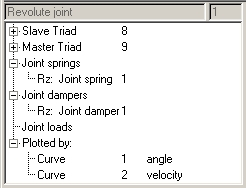
\includegraphics[width=0.4\textwidth]{Figures/ID_Topology window}
  \begin{picture}(135,0)
    \put( 60,105){\Bullet{1}}
    \put(120,105){\Bullet{2}}
    \put(-15, 60){\Bullet{3}}
  \end{picture}
\end{wrapfigure}

When an object in the model is selected, the ID and Topology panel
displays information related to the object as described below.
If multiple items are selected, only the item selected last is displayed.

\begin{bulletlist}
\item{\sl Item Type} --
  the type of the selected object (for example, Revolute joint, Gear, Spring).
\item{\sl ID Number} --
  a unique integer that distinguishes one item of the same type from another.
\item{\sl Topology view} --
  a list that displays the mechanism objects related or connected to
  the selected item.
\end{bulletlist}

\Tip{The Plotted by branch in the Topology view lists all curves that plot
  result quantities from the selected structural object.}

ID numbers are assigned automatically to new objects in numerical order.
If you delete an object such as a Ball joint with ID Number 3, this number
is free and the next Ball joint created is then assigned ID Number 3.

\subsubsection{Topology view and browsing}

Most mechanism components are related to other objects; for example, Joints
consists of Triads that are connected to Parts, and Sensors are measuring
variables from other mechanism components.

These relations are shown by the {\sl Topology} view in a hierarchical fashion,
indicating their topological relationships.
This list can then be used to investigate these related objects,
and to browse through the mechanism model through the topological connections.
This can be done by using the browsing features offered by the
{\sl Topology} view, as described below.

The items in the {\sl Topology} view will be highlighted in the {\sl Modeler}
view when you select an item keeping the mouse button pressed.
This is useful to see exactly which object in the 3D view that corresponds
to the listed item.

\begin{wrapfigure}{r}{0.25\textwidth}
  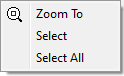
\includegraphics[width=0.25\textwidth]{Figures/2-TopologyViewPopupMenu}
\end{wrapfigure}

Right clicking an item in the {\sl Topology} view will show a tiny pop-up
menu that allows you to either \textbf{Zoom To} or \textbf{Select} the
item, or to do a \textbf{Select All}.

\clearpage
\begin{itemize}
\item\textbf{Zoom To}:
  This command zooms to the item making it easy to locate it in a complex model.
  See also \refSection{zoom-and-pan}{Zoom and Pan}.
\item\textbf{Select}:
  This command selects the right-clicked object from the {\sl Topology} view,
  and thus jump to it showing the properties of that item instead. See also
  \refSection{select}{Select} on how to get back to your previous selection.
\item\textbf{Select All}:
  This command will select all top-level objects currently in the
  {\sl Topology} view, but showing the properties of the last object only.
  The effect of this command is the same as doing a multi-selection from the
  {\sl Objects} list view of Model Manager panel using the \textbf{Shift} key,
  see \refSubSection{selecting-items}{Selecting items}{model-manager}.
\end{itemize}

\Tip{Double clicking an item in the Topology view will also select it.}


\SubSection{Property Editor}{property-editor}

The Property Editor panel is used to view and edit the properties
of mechanism items. The appearance of properties is different
depending on the object selected. The image below is an example
showing properties that are common to some of the Fedem modeling objects.

\begin{figure}[H]
  \begin{picture}(340,75)
    \put( 20, 0){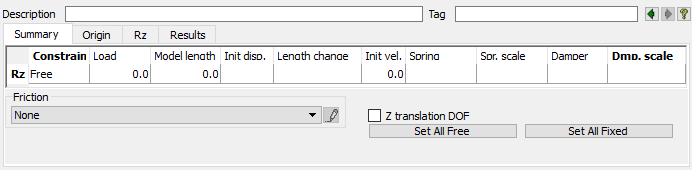
\includegraphics[width=0.9\textwidth]{Figures/2-PropertyPanel}}
    \put( 19, 0){\line(-1,0){7}}
    \put( 12, 0){\line(0,1){65}}
    \put( 12,65){\line(1,0){7}}
    \put( 50,65){\Bullet{1}}
    \put(240,65){\Bullet{2}}
    \put(307,56){\Bullet{3}}
    \put(318,56){\Bullet{4}}
    \put( -2,30){\Bullet{5}}
  \end{picture}
\end{figure}

\begin{bulletlist}
\item{\sl Description} --
  an optional user-supplied name or identifying remarks.
\item{\sl Tag} --
  an optional identifier which can be used to refer to the object from
  python scripts using the fedempy interface.
\item
\includegraphics[scale=0.5]{Figures/Icons/selectbackward}
  
\includegraphics[scale=0.5]{Figures/Icons/selectforward} --
  buttons for navigating back and forth through the latest selections
\item
\includegraphics[scale=2.0]{Figures/Icons/help} --
  help button that opens the Reference guide on the Property Editor guide
  content, depending on the type of the selected object.
\item{\sl Properties} --
  editable attributes specific to the selected object.
\end{bulletlist}

\Note{The description field may contain any ASCII-character,
  except for the “-character which is reserved for text string
  delimiters in the model file.}

\Note{The description field is also used to activate beta features,
  see \refAppendix{beta-feature-documentation}{Beta feature documentation}.}

\Caution{After editing a value in the Property Editor panel by typing,
  you must press the Enter key to apply the change.}

\subsubsection{Property menus}

\begin{wrapfigure}{r}{0.4\textwidth}
  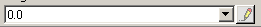
\includegraphics[width=0.4\textwidth]{Figures/2-PropertyValueMenu}
\end{wrapfigure}

Many mechanism items have internal properties that can depend on the
simulation time, measurement of a system variable or some internal
variable in the item in question. Property menus are used to
set up such properties in a simple way. These menus consist of
an option menu that in some cases are editable, and an \textbf{Edit} button.

\begin{wrapfigure}{r}{0.4\textwidth}
  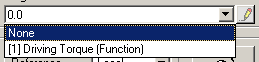
\includegraphics[width=0.4\textwidth]{Figures/2-PropertyValueMenu-Open}
\end{wrapfigure}

The menu contains references to other entities in your model
that can be used as input for the property in question.
A non-linear spring characteristic (e.g., a force-displacement curve)
will be listed in the stiffness property menu of an Axial spring,
Functions and Control outputs will be listed in the magnitude property menu
of a load, etc. Press the menu button to access the list.

\vskip\parskip
\IconText{pencilbutton}{By pressing the \textbf{Edit} button
  you will select the item shown in the menu, as if you had selected it in the
  Model Manager panel.
  This is a convenient way of navigating through the relations of the model,
  giving a simple way of finding the details of a complex model.}

In some of the property menus, a numeric value can be entered
instead of selecting a reference from the menu.
The spring stiffness property is a good example.
Entering a numeric value will assign that value as a constant spring
stiffness to the spring in question.

\Tip{Property menus that accepts a numeric value always have a numeric value
  as default, while “None” is normally the default for Property menus
  not accepting a number.}

To change a property from referring to a constant, select
the top entry in the pull-down list (which is either None
or the last numerical value that was entered in the same box),
or delete the current contents of the box, type in a numerical
value and then press Enter to apply the change.


\clearpage
\SubSection{Object Browser}{object-browser}

An alternative tool to display (but not edit) the detailed properties of
mechanism objects is via the Object Browser dialog box.

\IconText{objectBrowser}{It is opened by selecting \textbf{Objects Browser...}
  from the \textbf{Tools} menu, or from the right-click menu in the
  {\sl Objects} list view of the Model Manager panel.
  The Fedem Object Browser dialog box is shown below.}

\begin{figure}[H]
  \begin{picture}(340,277)
    \put(0,0){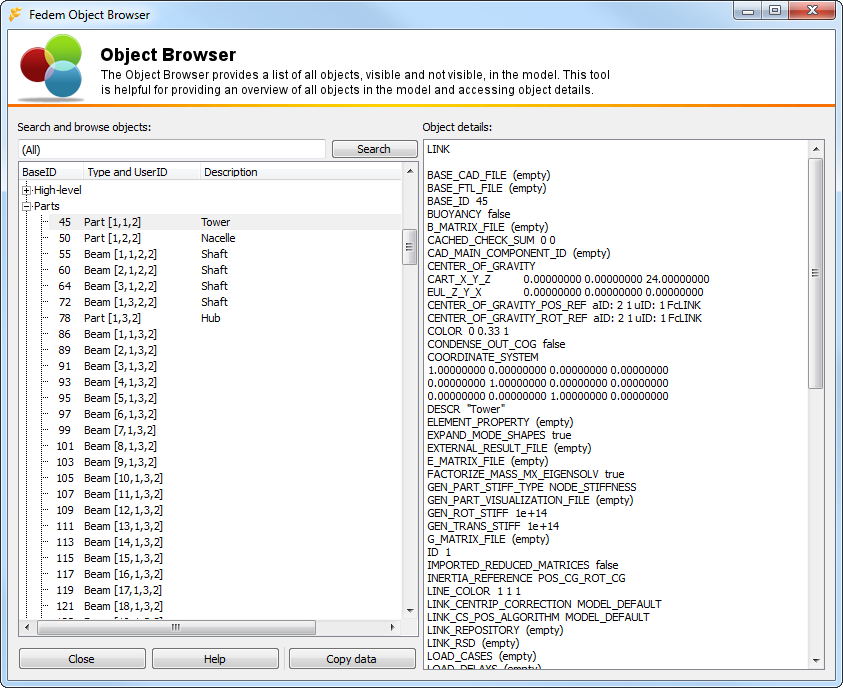
\includegraphics[width=\textwidth]{Figures/Dialogs/2-ObjectBrowser}}
    \put(16,213){\Bullet{1}}
    \put(47,213){\Bullet{2}}
    \put(90,213){\Bullet{3}}
    \put(205,220){\Bullet{4}}
  \end{picture}
\end{figure}

\begin{bulletlist}
\item{\sl BaseID} --
  This column lists the base ID of the objects.
  These are unique ID numbers over all objects in the model that are used for
  internal book-keeping only. They are not visible in the Fedem GUI elsewhere.
\item{\sl Type and UserID} --
  This column lists the type and user ID of the objects, which are used as
  unique identification of the objects elsewhere in the Fedem GUI.
  The user ID consists of a comma-separated list of values in brackets []
  when the object is part of a higher-level sub-assembly, see
  \refSection{user-id-convention}{User ID convention in assemblies}.
\item{\sl Description} --
  This column lists the description string of the objects.
\item{\sl Object details:} --
  This field lists in plain text all the information stored for the selected
  object in the model database. The formatting of this list resembles that of
  the model file (\File{.fmm}) itself.
  The first line contains the model file keyword for the selected object.
  Then the field name (in upper case) and value of each data field of that
  object (including also the base- and user ID and description found in the
  first three column) are listed in alphabetic order of the field name.
\end{bulletlist}

\Tip{The list in the left half of the Object Browser can be sorted with respect
  to the base ID, Type and User ID, or Description, by clicking on the
  respective column headings.}

When opened, the Object Browser dialog box
will display details for the currently selected object in the model. You can
also search for objects by typing their description in the search field and
clicking the search button. The Object Browser will list all objects in the
model if the search field is blank, or if no object was selected when the
dialog box was opened.

\Note{The Object Browser dialog box only displays objects that affect
  the numerical simulation of the model. Therefore, result objects
  (Graphs, Curves, Animations) as well as higher-level sub-assembly objects
  are not listed.}

The main purpose of the Object Browser dialog box is to provide an
overview of the keywords and field names used for the various object types
in the model file, as these are necessary for setting up the simulation events
when, for instance, a model consists of multiple load cases.
See \refSection{using-simulation-events}{Using simulation events}.


\SubSection{Workspace}{workspace}

The Workspace area is used for constructing, manipulating,
and viewing mechanism models, control systems, graphs and animations.
The Workspace can contain several views, including the {\sl Modeler},
{\sl Control Editor}, and multiple {\sl Graph} views.
These views are described in the following sections.

\Tip{The views in the Workspace can be managed using the
  \textbf{Tile} and \textbf{Cascade} commands from the \textbf{Windows} menu.}

\SubSubSection{Modeler}{modeler}

The Modeler view displays a 3D rendering of your mechanism and provides
dynamic viewing capabilities such as zooming, panning, and 2- and 3-dimensional
rotation (see \refSection{navigation}{3D Navigation}).
This view is also used to show animated simulation results.
Select the Modeler view to view, create, or edit a mechanism model.

\IconText{modeler}{To open the Modeler view, select \textbf{Show Modeler}
  from the \textbf{Windows} tool bar or menu.
  The {\sl Modeler} view is then displayed as shown below.
  See also \refSection{modeler-view}{Modeler view}.}

\begin{figure}[!h]
  \center
  \begin{picture}(293,193)
    \put(0,0){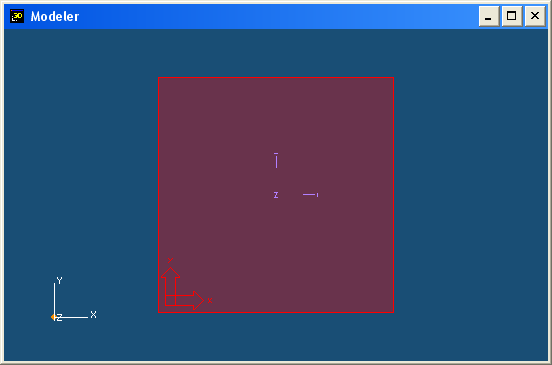
\includegraphics[width=0.85\textwidth]{Figures/2-Modeler}}
    \put(100,100){\Bullet{1}}
    \put(30,30){\Bullet{2}}
  \end{picture}
\end{figure}

\begin{bulletlist}
\item{\sl Reference Plane} --
  The shaded area in the center of the Modeler view represents a plane,
  which can be considered the ground or base for your models.
\item{\sl Global Directions} --
  The arrows located in the lower left corner of the Modeler view show the
  orientation of the global coordinate system and the direction of the
  gravity vector, $\bf g$.
\end{bulletlist}

\Tip{The Modeler view can be expanded to almost full screen size by hiding
  the Model Manager and Property Editor panels. To hide these panels,
  click the \textbf{Model Manager} and \textbf{Property Editor} buttons on
  the \textbf{Windows} tool bar (or from the \textbf{View} menu).
  Hiding the tool bars also increases the viewing area of the {\sl Modeler} view
  (see \refSubSection{manipulating-tool-bars}{Manipulating tool bars}
  {menus-and-tool-bars}).}
\begin{picture}(100,0)
  \put(-77,15){
\includegraphics[width=7mm]{Figures/Icons/modelManager}}
  \put(-49,15){
\includegraphics[width=7mm]{Figures/Icons/propertyPanel}}
\end{picture}

\subsubsection{Control Editor}

The Control Editor view is a workspace for editing the control system.
The graphical representation is a block-based diagram that consists of a series
of control blocks that can be connected to simulate your control system.
This editing environment allows you to create and manipulate the control system
using drag-and-drop functionality. It also features grid and snapping tools
(see \refSection{setting-grid-and-snap}{Setting Grid and Snap}).

\IconText{controlEditor}{To open the Control Editor view,
  click the \textbf{Show Control Editor} button on the \textbf{Windows} tool bar
  (or from the \textbf{Windows} menu). The Control Editor view
  displays the control system (an example is shown below).
  See \refChapter{control-system-modeling}{Control System Modeling}
  for more information on the topic.}

\begin{figure}[H]
  \center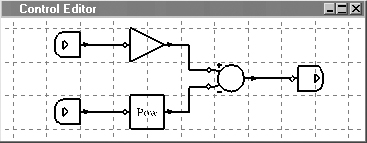
\includegraphics[width=0.8\textwidth]{Figures/cs_example}
\end{figure}

\Note{The Control Editor view is empty until you create control elements.}

\subsubsection{Graph Views}

The Graph view can display various graphed results. You can customize graphs
of selected simulation results and manipulate the Graph view.

\IconText{graphGroup}{To open a Graph view, right-click the Graph from the
  {\sl Results} list of the Model Manager panel, and select \textbf{Show Graph}.
  The Graph views are displayed in the Workspace area as shown below.}

\begin{figure}[H]
  \center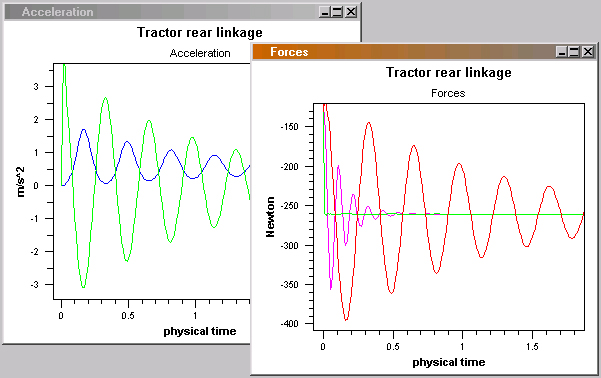
\includegraphics[width=0.86\textwidth]{Figures/graphsCOLOR}
\end{figure}


\def\OutputList{\protect\hyperlink{output-list}{\sl Output List}~}
\SubSection{Output List}{output-list}

The Output List view displays written output from Fedem,
such as a log of commands and solver executions, and error messages.
%This view allows you to observe the commands performed by Fedem.

\vskip\parskip
\IconText{outputList}{To open the Output List view,
  select \textbf{Show Output List} from the \textbf{Windows} menu or tool bar.}

\begin{figure}[H]
  \center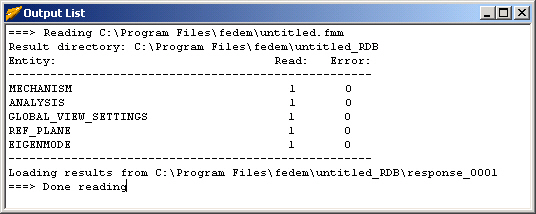
\includegraphics[width=0.8\textwidth]{Figures/Output_List_window_COLOR}
\end{figure}

The text in the Output List view is also written to a log file.
The name of this log file is the same as the current model file name,
but with extension \File {.log} instead of \File{.fmm}.
Therefore, a new log file is opened whenever you \textbf{Open} a
new model, or perform a \textbf{Save As...} command.

\Note{If a log file already exists for the model you open from an earlier
  Fedem session, the output from the current session is appended to that file.
  That means that the entire history of the Output List content for the model
  is recorded. In addition, the date and time of the model open and close
  operations, as well as the Fedem version used, are recorded to the log-file.}


%%%%%%%%%%%%%%%%%%%%%%%%%%%%%%%%%%%%%%%%%%%%%%%%%%%%%%%%%%%%%%%%%%%%%%%%%%%%%%%%
\Section{Executing commands}{executing-commands}

\hskip-33mm
\begin{minipage}{1.4\textwidth}
  \begin{tabular}{p{0.16\textwidth} p{0.49\textwidth} p{0.35\textwidth}}
    \vspace{0pt} 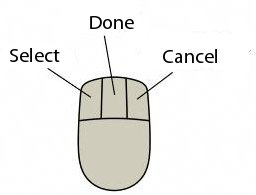
\includegraphics[width=25mm]{Figures/2-mousebuttons} &
    \vspace{0pt} \raggedright
    When performing commands in Fedem, the Guide panel prompts you
    with instructions for completing each command. You may be asked to select
    mechanism objects or locate points to place or move objects.
    Performing commands makes use of three actions:
    \textbf{Select}, \textbf{Done} and \textbf{Cancel}. &
    \vspace{0pt} 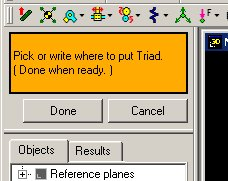
\includegraphics[width=32mm]{Figures/2-Guide}
  \end{tabular}
\end{minipage}

\SubSection{Select}{select}

To select items in your model, or points on objects as references for
moving or creating items, place the cursor over the object or position
and press the left mouse button (left-click). The item is highlighted
and its properties can then be edited in the Property Editor panel.

\Note{Some commands require that an object is selected from views in the
  Workspace area only, such as the Modeler or Control Editor views.
  Instructions regarding these commands are provided in the Guide panel.}

\Tip{To deselect an item, simply click an empty space within the Modeler view.}

\subsubsection{Snapping}

When selecting objects in your model, the selection automatically snaps to
a point on the object such as the nearest node on an FE part, the center point
of a joint, and so on. This makes your selection quick and accurate.

Snapping behaves differently on different types of objects. FE parts, VRML
models, CAD parts and mechanism symbols all have different snapping policies.
Selection snaps to FE nodes on FE parts, to vertices on a VRML part,
to geometry features such as center points and edges on CAD parts,
and to important points on other mechanism symbols.

\subsubsection{Multiple selection}

Some Fedem commands, such as \textbf{Smart Move} and \textbf{Delete},
allow you to select several items at once. To select more than one item,
press and hold down the \textbf{Ctrl} key and then click the items you want
to add to your selection.

If you accidentally add the wrong object to the selection, simply
release the Ctrl key and click an empty space within the Modeler view.
The last selected item is deselected.

\subsubsection{Selection history}

Fedem maintains a history of the items you have selected suring the current
session, which can be accessed using the \textbf{Select Backward} and
\textbf{Select Forward} commands:

\vskip\parskip
\IconText{selectbackward}{To choose a previous selection,
  press the \textbf{Select Backward} button.
  You may need to press it several times to cycle back through the selections
  until the desired object or selection is reached.}

\IconText{selectforward}{To select a recent selection,
  press the \textbf{Select Forward} button once or as many times as necessary
  until the desired selection is reached.}

\subsubsection{Co-located items}

Sometimes several items in a model are located very close together or
on top of each other; in Fedem, these are called co located items.
To select a co located item, click the same spot several times to
cycle through the items. Fedem cycles from the item closest to the viewer to
the one furthest from the viewer.

\subsubsection{Selection Filter}

Some Fedem commands allow you to select only certain types of items.
These restrictions are automatically imposed and based on the type
of command in use. For example, sensors cannot be applied directly to
parts, and Fedem will therefore limit your selection to other types
of mechanism items. To make the selection even easier, you can also
filter the selectable items by limiting the types of items displayed
in the {\sl Modeler view}.

\Tip{To limit the display of mechanism objects, click the
  \textbf{General Appearance} button on the \textbf{Standard} tool bar,
  then disable Mechanism symbols as necessary.
  (See also \refSection{general-appearance}{General Appearance}.)}

\subsubsection{Selecting ground}

To select the ground during modeling,
simply click anywhere on the Reference Plane.

\SubSection{Done}{done}

When executing a command in Fedem, the Guide panel prompts you to select
items or locate points. When you have achieved the desired selection, press
the \textbf{Done} button in the Guide panel to accept it.

\Tip{You can also press the center mouse button within one of the Workspace
  views or the \textbf{Enter} key on the keyboard to accept the selection.}

\SubSection{Cancel}{cancel}

To abort or escape a command procedure,
press the \textbf{Cancel} button on the Guide panel.

\Tip{You can also press the right mouse button within one of the Workspace views
  or the \textbf{Esc} key on the keyboard to cancel a command.}


%%%%%%%%%%%%%%%%%%%%%%%%%%%%%%%%%%%%%%%%%%%%%%%%%%%%%%%%%%%%%%%%%%%%%%%%%%%%%%%%
\Section{Visualizing the model}{visualizing-the-model}

\SubSection{3D Navigation}{navigation}

The 3D navigation commands enables you to change the view without interrupting
the current command or procedure.
There are several different sets of viewpoint control commands:

\begin{itemize}
\item Middle mouse button/wheel + mouse motion
\item Function keys (\textbf{F1}, \textbf{F2}, \textbf{F3}
  and \textbf{F4} + mouse motion)
\item Keyboard keys
\item Predefined view tool buttons
\end{itemize}

\subsubsection{Middle mouse button/wheel}

Pressing and holding the middle mouse button (or wheel if your mouse have that)
while moving the mouse will rotate the view around the rotation center.
If the button/wheel was pressed near the edge of the 3D view, the rotation will
be restricted to the viewport’s normal axis.
Rolling the mouse wheel will zoom in and out. When the mouse wheel is used to
zoom in, the view will be zoomed towards the position of the mouse pointer
giving a combined zoom and pan behavior.
Using the middle mouse button commands is the mostly used 3D navigation method.

\subsubsection{Function keys}

The function key based navigation can be used when you need added control
over the navigation. The commands include:

\begin{itemize}
\item Pan 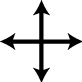
\includegraphics[scale=0.7]{Figures/pan} (\textbf{F1})
\item Zoom 
\includegraphics[scale=0.7]{Figures/zoom} (\textbf{F2})
\item Rotate 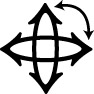
\includegraphics[scale=0.7]{Figures/rotate} (\textbf{F3})
\item Select rotation center
  
\includegraphics[scale=0.7]{Figures/rotate_center} (\textbf{F4})
\end{itemize}

%These functions are often useful while working in the Modeler view.
%We recommend that you keep your left hand near these function keys while you work.

To use the function key commands, press and hold the function key,
and move the mouse to manipulate the view. The manipulation will only occur
as long as the mouse is inside the Modeler view.
By pressing the left mouse button, you may avoid this restriction.
When the function key is released, the manipulation stops.

\Caution{When pressing the left mouse button while using the function keys,
  Fedem grabs the mouse and keyboard control.}

\subsubsection{Pan - (F1)}

The Pan 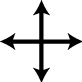
\includegraphics[scale=0.7]{Figures/pan} command shifts the view left,
right, up or down.

\subsubsection{Zoom - (F2)}

The Zoom 
\includegraphics[scale=0.7]{Figures/zoom} command moves the scene
closer or further away from the camera.
It pays attention to the rotation center, and will zoom towards it
(see \protect\hyperlink{select-rotation-center}{\sl"Select rotation center (F4+Select)"} below).
This is useful when you need to examine an object or its components closely.

\Tip{To achieve maximum zoom at a specific point, select the point using
  Select rotation center (\textbf{F4}) and then zoom in on the point using
  Zoom (\textbf{F2}).}

\subsubsection{Rotate - (F3)}

The Rotate 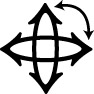
\includegraphics[scale=0.7]{Figures/rotate} command enables you to
dynamically rotate your model around a point or an axis at the rotation center
(see \protect\hyperlink{select-rotation-center}{\sl"Select rotation center (F4+Select)"} below).
The rotation can be performed in two different ways, depending on the position
of the cursor when you press \textbf{F3}.

\begin{itemize}
\item Axis rotation: With the cursor near the edge of the {\sl Modeler view},
  the model rotates around an axis that is perpendicular to the screen.
\item Point Rotation: With the cursor near the center of the view,
  the model rotates around a point located at the rotation center
  some distance into the model. This allows rotation of the model
  in any direction around the point.
\end{itemize}

\Tip{The rotation motion is sensitive to the speed of the mouse.
  If the mouse is moved slowly the control of the rotation becomes finer, and
  makes it possible to accurately control the view along long constructions.}

\SubSubSection{Select rotation center (F4+Select)}{select-rotation-center}

The Select rotation center 
\includegraphics[scale=0.7]{Figures/rotate_center}
command enables you to select a new center for zooming and rotation.
When you use \textbf{F4} to select a point, the selected target point shifts to
the center of the view and becomes the new dynamic center used by the Zoom
(\textbf{F2}) and Rotate (\textbf{F3}) commands.
This target point remains the dynamic center until the model is moved
by some other viewing command.

To select a new rotation point, press and hold down the \textbf{F4} key,
move the cursor to the target point, and click the left mouse button.

\Tip{To closely examine a part of your model, set the dynamic center
  (\textbf{F4}) at the point of interest, and use Zoom (\textbf{F2})
  to magnify the view.
  You can then easily examine the point from many directions using Rotate
  (\textbf{F3}).}

\subsubsection {Keyboard keys}

To rotate the model by increments of 15 degrees, use the arrow keys.
Rotation and panning may also be done by pressing \textbf{Shift}
(rotate 90 degrees), \textbf{Alt} (rotate around screen normal) or
\textbf{Ctrl} (panning) in combination with arrow keys.
To zoom in and out, press \textbf{z} or \textbf{Shift + z}.


\SubSection{Predefined view tool buttons}{predefined-view-tool-buttons}

Fedem provides the following commands for some predefined view settings:

\vskip\parskip
\IconText{isometricView}{\textbf{Isometric}\newline
  To display an isometric view of your mechanism, click the \textbf{Isometric} button.}

\vskip\parskip\IconText{viewTop}{\textbf{Top}\newline
  To display the top view of your mechanism, click the \textbf{Top} button.}

\vskip\parskip\IconText{viewRight}{\textbf{Right}\newline
  To display the side view of your mechanism, click the \textbf{Right} button.}

\vskip\parskip\IconText{viewFront}{\textbf{Front}\newline
  To display the front view of your mechanism, click the \textbf{Front} button.}

\vskip\parskip\IconText{viewBottom}{\textbf{Bottom}\newline
  To display the bottom view of your mechanism, click the \textbf{Bottom} button.}

\vskip\parskip\IconText{viewLeft}{\textbf{Left}\newline
  To display the left side view of your mechanism, click the \textbf{Left} button.}

\vskip\parskip\IconText{viewBack}{\textbf{Back}\newline
  To display the back view of your mechanism, click the \textbf{Back} view button.}


\SubSection{3D View Controls}{view-controls}

Fedem provides several 3D viewing commands for use in the {\sl Modeler} view.
The following commands can be accessed on the {\textbf 3D View Control} tool bar
(or from the \textbf{View} menu):

\vskip\parskip\IconText{solidView}{\textbf{Solid View}\newline
  To display all mechanism items as solid/shaded objects,
  click the \textbf{Solid View} button. This is on by default.}

\vskip\parskip\IconText{lineView}{\textbf{Line View}\newline
  To speed up graphic performance and display all mechanism items as outlines,
  click the \textbf{Line View} button.}

\vskip\parskip\IconText{flatShading}{\textbf{Flat Colors}\newline
  To render the model without shading, click the \textbf{Flat Colors} button.
  This is especially useful when viewing color plots.
  This option is off by default.}

\vskip\parskip\IconText{showTopFaces}{\textbf{Show Top Faces}\newline
  To distinguish the top and bottom faces of shell elements,
  click the \textbf{Show Top Faces} button. The top faces will then be rendered
  normally while the bottom faces will be rendered dark/black. If some of the
  parts have the detail level set to Reduced Surface or Reduced Surface and
  Internals, only a rough indication on the states of the faces is given.
  To see the exact top and bottom of every face on a part, set the detail level
  to Surface or Surface and Internals. This is off by default.}

\vskip\parskip\IconText{perspectiveView}{\textbf{Perspective}\newline
  To display a perspective view of your mechanism,
  click the \textbf{Perspective} button. This command controls the appearance
  of mechanisms in depth as perceived by normal binocular vision.}

\vskip\parskip\IconText{parallelView}{\textbf{Parallel Projection}\newline
  To display a parallel view of your mechanism,
  click the \textbf{Parallel Projection} button.}


\SubSection{Zoom and Pan}{zoom-and-pan}

Fedem provides zooming and panning controls for use in the active view.
The following commands can be accessed on the \textbf{Zoom and Pan} tool bar
(or from the \textbf{View} menu):

\Note{Some of these commands cannot be used in all views.
  When commands cannot be used in the current view, their buttons become
  unavailable (grayed out) on the menus and tool bars.}

\vskip\parskip\IconText{zoomAll}{\textbf{Zoom All}\newline
  To scale the active view so that all objects (for {\sl Graph} views,
  every Curve on the Graph) fit within the view, press the \textbf{Zoom All}
  button. When working in {\sl Graph} views, this can also be achieved by
  pressing the \textbf{F5} key.}

\vskip\parskip\IconText{zoomWindow}{\textbf{Zoom Window}\newline
  To enlarge a rectangular area, press the \textbf{Zoom Window} button.
  The command can also be activated by pressing the \textbf{Z} key.}

\vskip\parskip\IconText{zoomTo}{\textbf{Zoom To}\newline
  This command pops up the correct view, zooms to the selected object,
  and places the Dynamic Center of rotation at the center of the object.
  This is useful when trying to locate a certain Triad or Joint in large models.
  This command is also available from the {\sl Topology} view and the
  Model Manager panel (see \refSection{model-manager}{Model Manager}
  and \refSection{id-and-topology-panel}{ID and Topology panel}).
  It is also applicable on Control Elements and Control Lines in the
  {\sl Control Editor} view (see \refSection{control-editor}{Control Editor}).}

% This feature vanished with the Qwt-porting years ago
%\vskip\parskip\IconText{zoomWindowAutoscale}{
%  \textbf{Zoom Window with Autoscale}\newline
%  To enlarge a rectangular area, press the \textbf{Zoom Window With Autoscale}
%  button. The contents will be auto scaled to fit the entire plotting area.
%  This command can also be activated by pressing the \textbf{X} key.}

\vskip\parskip\IconText{zoomIn}{\textbf{Zoom In}\newline
  To enlarge the active view by a predefined scale factor,
  press the \textbf{Zoom In} button.}

\vskip\parskip\IconText{zoomOut}{\textbf{Zoom Out}\newline
  To reduce the active view by a predefined scale factor,
  press the \textbf{Zoom Out} button.}

\vskip\parskip\IconText{panLeft}{\textbf{Pan Left}\newline
  To move the active view to the left, press the \textbf{Pan Left} button.}

\vskip\parskip\IconText{panRight}{\textbf{Pan Right}\newline
  To move the active view to the right, press the \textbf{Pan Right} button.}

\vskip\parskip\IconText{panUp}{\textbf{Pan Up}\newline
  To move the active view up, press the \textbf{Pan Up} button.}

\vskip\parskip\IconText{panDown} {\textbf{Pan Down}\newline
  To move the active view down, press the \textbf{Pan Down} button.}


\SubSection{General Appearance}{general-appearance}

The \textbf{General Appearance} command can be used to control which entities
are displayed in the {\sl Modeler} view. This command also provides control of
the size and appearance of mechanism symbols.

\vskip\parskip
\IconText{generalAppearance}{Click the \textbf{General Appearance} button
  to open the associated dialog box (shown below).}

\clearpage
\noindent
\begin{minipage}{0.6\textwidth}
  \raggedright
  \begin{bulletlist}
  \item{\sl Mechanism symbols} --
    allows you to toggle on/off the display of mechanism items
    of different type, to edit the color used to specify each item type,
    and to change the size of symbols and line width
    (see \protect\hyperlink{mechanism-symbols}{\sl"Mechanism symbols"} below).
  \item{\sl Default colors} --
    controls the colors used for Grounded Triads,
    unattached mechanism items and the Modeler background
    (see \protect\hyperlink{default-colors}{\sl"Default colors"} below).
  \item{\sl Viewer options} --
    controls 3D rendering options such as visibility, transparency type,
    and line-smoothing
    (see \protect\hyperlink{viewer-options}{\sl"Viewer options"} below).
  \end{bulletlist}
\end{minipage}% <--- the % is needed here to kill off  spurious spacing
\begin{minipage}{0.4\textwidth}
  \raggedleft
  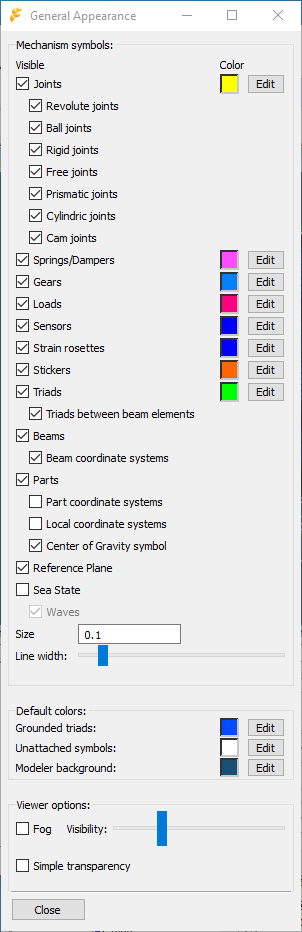
\includegraphics[trim=0 400 0 0,clip,scale=0.55]{Figures/Dialogs/2-GeneralAppearance}
\end{minipage}

\SubSubSection{Mechanism symbols}{mechanism-symbols}

This area provides the following controls:

\noindent
\begin{minipage}{0.6\textwidth}
  \raggedright
  \begin{itemize}
  \item{\sl Visible} --
    enables/disables the display of each item type.
    Click the box next to an item type to change the setting. The toggles that
    are indented slightly to the right are considered as sub-types of the item
    toggle just above them. They are active only if that toggle is enabled.
    \vskip1mm
    \MiniGenericNote{tip}{TIP}{-30mm}{1.83}{0.173}{0.48}{
      Turning off visualization of items speeds up and simplifies the display
      of complex mechanisms, and provides a useful way to limit the selection
      to specific item types.}
  \end{itemize}
\end{minipage}% <--- the % is needed here to kill off spurious spacing
\begin{minipage}{0.4\textwidth}
  \raggedleft
  \begin{picture}(125,173)
    \put(0,0){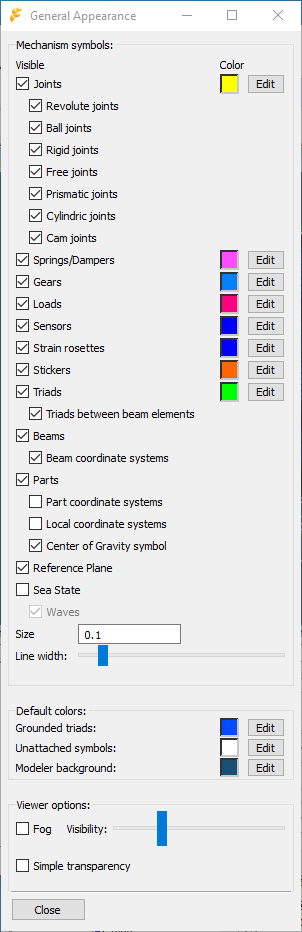
\includegraphics[trim=0 0 0 300,clip,scale=0.55]{Figures/Dialogs/2-GeneralAppearance}}
    \put(-10,362){\Bullet{1}}
    \put(-10,87){\Bullet{2}}
    \put(-10,47){\Bullet{3}}
  \end{picture}
\end{minipage}

\noindent
\begin{minipage}{0.6\textwidth}
  \raggedright
  \begin{itemize}
  \item{\sl Color} --
    allows editing of the RGB settings for each item type.
    Press the \textbf{Edit} button next to an item type to edit the default
    display color for that item type. In the appearing dialog box
    (shown at right), move the sliders to change the settings or enter
    the desired values directly in the number fields.
  \end{itemize}
\end{minipage}% <--- the % is needed here to kill off spurious spacing
\begin{minipage}{0.4\textwidth}
  \raggedleft
  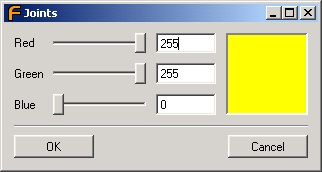
\includegraphics[scale=0.52]{Figures/Dialogs/2-Color}
\end{minipage}

\clearpage
\begin{itemize}
\item{\sl Size} --
  a scale factor for sizing the display of mechanism entities.
  To change the size of items, enter a new number in the size field.
\item{\sl Line Width} --
  this is a scale factor for the line width of all mechanism symbol lines,
  together with all 1D elements and Surface Connectors in the FE parts
  (see \refSection{surface-connectors}{Surface Connectors}).
  To change the line-width, move the slider right or left.
\end{itemize}

\SubSubSection{Default colors}{default-colors}

This area enables the user to edit the colors used on the modeling background
and unattached mechanism items. It also allows you to set the colors on Triads
that are attached to the Ground, to distinguish them from Triads that are free
to move. The default colors may be changed in a similar ways as changing the
colors for \protect\hyperlink{mechanism-symbols}{\sl Mechanism symbols}.

\SubSubSection{Viewer Options}{viewer-options}

This area enables the user to modify the way that models are rendered.

\begin{itemize}
\item{\sl Fog} is an option that enables you to create a fog-like effect around
  your model that appears as fog or darkness (or even an underwater scene).
  The distant parts of the model appear to fade into the background.
  The Visibility slider controls the distance at which the model is completely
  hidden in the fog.
 \item{\sl Simple Transparency} is a dithering algorithm used to speed graphic
   performance when displaying transparent objects in your model.
   The effects of this option depend on the type of graphics card you have.
 \item{\sl Anti-Aliasing} enables/disables line-smoothing for symbols.
\end{itemize}

\Tip{You can create the following effects with the Fog option:
  \begin{itemize}
  \item To create the effect of a foggy day, set the Modeler background color to
    light gray (Red 180, Green 180, Blue 180), enable the Fog option, and adjust
    the Visibility slider until the model almost fades into the background.
  \item To create the effect of an underwater scene, set the Modeler background
    color to sea green (Red 20, Green 125, Blue 130), enable the Fog option,
    and adjust the Visibility slider until the model nearly
    fades into the background.
  \end{itemize}}

\Tip{If Anti-Aliasing does not function properly,
  try enabling the Simple Transparency option.}

\Note{Graphics cards do not all have the same optimal settings.
  In general, disabling the Fog and Anti-Aliasing options and turning on
  Simple Transparency gives the best performance, but with some systems the
  performance gain is insignificant.}


\SubSection{Item Appearance}{item-appearance}

The \textbf{Item Appearance} command can be used to change the level of detail
and the appearance of individual Parts and the Reference Plane.

\IconText{itemAppearance}{To open the Item Appearance dialog box (shown below),
  click the \textbf{Item Appearance} button on the \textbf{Standard} tool bar,
  and select a Part or the Reference Plane for which you want to change the
  appearance of.}

\Tip{To change the appearance of a hidden Part, select the Part in the
  {\sl Objects} list of the Model Manager panel, after clicking the
  \textbf{Item Appearance} button.}

\noindent
\begin{minipage}{0.55\textwidth}
  \raggedright
  \begin{bulletlist}
  \item{\sl Level of Detail} --
    controls the level of complexity displayed in the model.
    The {\sl Polygons} and {\sl Lines} settings allow you to change
    the complexity of models displayed in the {\sl Modeler} view,
    (see \protect\hyperlink{level-of-detail}{\sl"Level of Detail"} below).
    Changing these settings can improve the graphic performance of 3D rendering.
  \item{\sl Color} --
    controls the RGB settings of the selected Part or Reference Plane.
  \item{\sl Material} --
    controls the shininess and transparency of the selected Part
    or Reference Plane.
  \end{bulletlist}
\end{minipage}% <--- the % is needed here to kill off spurious spacing
\begin{minipage}{0.45\textwidth}
  \raggedleft
  \begin{picture}(136,180)
    \put(0,0){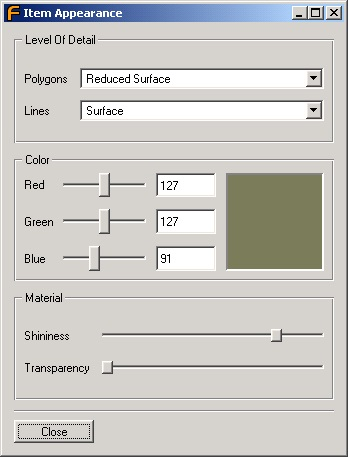
\includegraphics[scale=0.52]{Figures/Dialogs/2-ItemAppearance}}
    \put(-5,158){\Bullet{1}}
    \put(-5,112){\Bullet{2}}
    \put(-5,56){\Bullet{3}}
  \end{picture}
\end{minipage}

\SubSubSection{Level of Detail}{level-of-detail}

Polygons can be displayed at five levels of detail:
Surface and Internals, Reduced Surface and Internals,
Surface, Reduced Surface, and Off. The default level is Surface.

\begin{enumerate}
\item{\sl Surface and Internals} --
  With polygon detail set to Surface and Internals,
  element faces from solid elements inside the parts are shown
  together with the surface faces of the elements.
  All element faces are shown as single polygons.
\item{\sl Reduced Surface and Internals} --
  Setting the detail level to Reduced Surface and Internals displays
  a simplified polygon representation of the surface and internals of a part.
  This is faster than using Surface and Internals,
  but shows a less accurate representation of the parts.
\item{\sl Surface} --
  This option turns off the internal faces in a part,
  and will only show the surface element faces of a part.
  All the surface faces are shown as separate polygons.
\item{\sl Reduced Surface} --
  Setting the polygon detail to Reduced Surface provides the most efficient way
  to visualize the shaded view of a mechanism part.
  The surface is displayed using a simplified polygon model
  and the internal faces are turned off.
\item{\sl Off} --
  Setting the polygon detail to Off turns all polygons off.
\end{enumerate}

Lines can be displayed at six levels of detail: Full, Surface, Outline, Outline
No 1D-elements, Simplified, and Off. The default level is Outline.

\begin{enumerate}
\item{\sl Full} --
  With line detail set to Full, mesh lines from solid elements inside the parts
  are shown together with the surface mesh of the elements.
\item{\sl Surface} --
  Setting the line detail level to Surface displays only the mesh lines
  on the surface of the FE model.
\item{\sl Outline} --
  This option leaves only the mesh lines on the surface of the part with
  neighboring element faces with a relative face-angle above a given threshold.
  The default threshold is $\pi/4$. (It is possible to edit this
  value for each part by editing the model file.)
\item{\sl Outline No 1D-elements} --
  Same as {\sl Outline} except that all Surface Connectors and 1-D elements,
  such as RGD, WAVGM, BEAM2, are also removed from the display.
\item{\sl Simplified} --
  This option generates a simple line visualization of the part
  based on the Triads attached to it.
  One line is drawn from each Triad to their geometrical center.
  This option makes most sense if the polygons are turned off.
  This visualization is the same that is used if the part is not loaded,
  see \refSection{fe-data-settings}{FE-Data Settings}.
\item{\sl Off} --
  Setting the line detail to Off turns all mesh lines off.
\end{enumerate}

\Tip{To edit the appearance or level of detail on several parts
  at the same time, select multiple parts in the Objects list in the
  Model Manager panel, after clicking on the Item Appearance icon.}


\SubSection{Element face visibility}{element-face-visibility}

The visibility of elements can be controlled using the commands
\textbf{Hide Element Faces} and \textbf{Show Element Faces} in the right-click
menu in the {\sl Objects} list of the Model Manager panel.
These commands can be applied to the entire part, or to a selection of the
element groups listed in the {\sl Objects} list.
The icon in front of each group entry in the list indicates the current visual
state of the elements in that group:
Either all visible 
\includegraphics[scale=0.8]{Figures/AllElementsVisible},
some visible 
\includegraphics[scale=0.8]{Figures/SomeElementsVisible}
or all hidden 
\includegraphics[scale=0.8]{Figures/AllElementsHidden}.

These commands will only be active when the polygon detail level is set to
Surface or Surface and Internals, or when color contour results are loaded for
the Part. This feature can also be utilized to load color contour results only
for small parts of a big Part because the color values will not be loaded on
hidden elements. See also
\refSection{performance-of-animation-loading}{Performance of animation loading}.

\Note{The visibility of the mesh is not affected by the
  \textbf{Show}/\textbf{Hide} commands.}


\SubSection{Visualization of special elements}{visualization-of-special-elements}

There are several element types that are treated differently from normal elements
like shells and solids, when it comes to visualization. Those elements are
listed in the table below.

\begin{table}[h!]
\begin{tabular}{ | m{33mm} | m{25mm}| m{45mm} | }
 \hline
 Element type & Visualization & Comments \\
 \hline\hline
 Beams & Dash dot lines & Any eccentricity is shown as dotted lines from the nodal point to the beam end \\
 \hline
 Rigid bars & Dashed lines & \\
 \hline\raggedright
 Constraint elements (RBE3, WAVGM, Distributed coupling) & Dotted lines &  \\
 \hline
 Concentrated mass & No visualization & \\
 \hline
 Springs & No visualization &  \\
 \hline
 Bush elements & No visualization & \\
 \hline
\end{tabular}
\end{table}

\subsubsection{Color}

The color of those elements are set automatically to black, white or a
grayish color to achieve a good contrast to both the color of the part,
and the viewer background. If the FE part is displayed using lines only,
the color of those elements is set to the color of all the other lines.

\subsubsection{Line width}

The line width is adjusted according to the Line Width parameter set
for the Mechanism symbols.
See \refSection{general-appearance}{General Appearance}.


\SubSection{Measuring distance and angles in a model}{measuring-distance-and-angles}

Sometimes during the modeling of complex mechanisms, it is necessary or
convenient to quickly assess the distance between two arbitrary points
in the model or to measure the angle between two lines. For this purpose,
two command are available from the \textbf{Tools} menu.

\vskip\parskip
\IconText{distance}{Select \textbf{Measure distance...} to check the
  distance between two points. Then click on two points in the {\sl Modeler}
  view to output their global positions and the relative distance between them
  in the \OutputList view.
  You can repeat to click on two new points to check their relative
  distance as many times you like. Press \textbf{Cancel} to quit the command.}

\begin{figure}[H]
  \center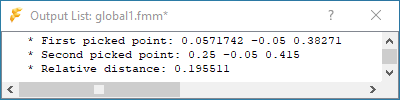
\includegraphics[scale=0.8]{Figures/2-OutputListDistance}
\end{figure}

\IconText{angle}{Select \textbf{Measure angle...} to check the
  angle between two lines defined through three selected points.
  The end points of the two lines are selected first by clicking on two
  arbitrary locations in the {\sl Modeler} view, followed by the common start
  point of the two lines.
  The global positions of the three selected points, as well as the angle
  (in radians) rotating the line though the third and first point into the line
  through the third and second are then shown in the \OutputList view.
  You can repeat to click on three  new points to measure more angles as many
  times you like. Press \textbf{Cancel} to quit the command.}

\begin{figure}[H]
  \center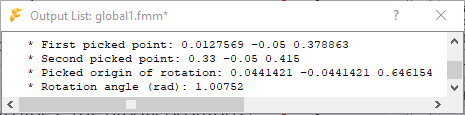
\includegraphics[scale=0.7]{Figures/2-OutputListAngle}
\end{figure}


%%%%%%%%%%%%%%%%%%%%%%%%%%%%%%%%%%%%%%%%%%%%%%%%%%%%%%%%%%%%%%%%%%%%%%%%%%%%%%%%
\Section{Opening and saving model files}{opening-and-saving-model-files}

\SubSection{Opening a file}{opening-a-file}

You can open a Fedem model file created in this version
(or any of the previous versions) of Fedem through the following steps:

\vskip\parskip
\IconText{open}{\vskip-5mm
  \begin{enumerate}
  \item Chose \textbf{Open...} in the File menu,
    or use the \textbf{Open} icon in the tool bar,
    to make the Open model file dialog box appear (shown below).
  \item Locate the wanted Fedem model in the dialog box and click \text{Open}.
\end{enumerate}}
\vskip-5mm

\begin{figure}[H]
  \center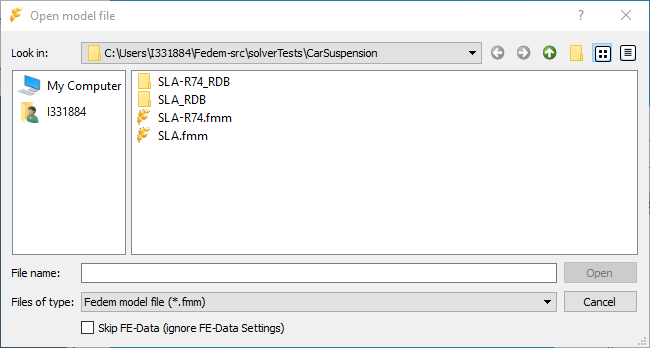
\includegraphics[scale=0.62]{Figures/Dialogs/2-Open}
\end{figure}

The Open model file dialog box normally displays all files with the Fedem model
file extension (\File{.fmm}). However, you may open a file with any extension by
selecting the All files filter in the File of type pull-down menu.

\Caution{If you choose to open a file without the \File{.fmm} extension,
  you should make sure it is a proper Fedem model file.
  Attempting to open a non-model file will usually result in an empty model,
  but unpredictable behavior may also occur, depending on the actual contents
  of the file.}

You can skip the loading of FE data for the parts if the model contains
large parts that take a long time to load. See also
\refSection{skipping-fe-data-when}{Skipping FE-Data when opening a model file}.

If the opened model file contains results, information about the
result files in the model (.frs files) is reported in the \OutputList view.
However, results files belonging to unloaded parts
(see \refSection{loading-and-unloading-fe-data}{Loading and unloading FE-Data})
and disabled result files
(see \refSection{result-manipulation}{Result manipulation})
are not included in this report.

If any problems are encountered during model loading, Fedem displays
a message box and provides additional information in the \OutputList view.

\Note{There might be minor changes in the model file format from one
  Fedem version to subsequent versions of Fedem.
  The newer versions are always backward compatible such that you may
  safely open a model that was created in one particular version in any
  of the subsequent versions, without loosing model consistency.
  The model is automatically converted to the new format while reading it.}

\Caution{The Fedem model files are not necessarily forward compatible.
  If you open a model in an older version of Fedem than it was created in,
  there might be changes in the model file format that makes the imported model
  incorrect or inconsistent.
  In some cases it may also make the Open operation fail or hang.
  Refer to the Fedem R5.0 Release Notes, Chapter 3, "Notes",
  for a summary of the forward compatibility issues that might need to
  be manually resolved in such cases.}

\subsubsection{Loading parts}

When Fedem opens a model file and the loading of FE data is enabled,
the part information (\File{.ftl} files, reduced matrix files, etc.)
is read from the FE model repository,
see \refSection{using-fe-model-repositories}{Using FE model repositories}.

If the FE model repository is missing, for example when a model
file is moved, Fedem uses the following search path to locate the parts:

\begin{enumerate}
\item The name and location of the originally imported FE part.
\item The name of the original FE part, located in a sub-directory
  of the current model file directory, with the same name as in the
  original FE file path (only if the original path was an absolute path).
\item The name of the original FE part, located in a parallel
  directory of the current model file directory, with the same name as in the
  original FE file path (only if the original path was an absolute path).
\item The name of the original FE part, located in the same
  directory as the model file.
\item The base name of the original FE part with the extension \File{.ftl}
  located in the same directory as the model file.
\end{enumerate}

\clearpage
\SubSection{Saving models}{saving-models}

To save the current model, do one of the following:

\vskip\parskip
\IconText{save}{\vskip0pt
  \begin{itemize}
  \item To replace the current version on disk,
    choose \textbf{Save} in the \textbf{File} menu or
    click on the \textbf{Save} icon in the tool bar.
  \item To save the file in a different location and/or with a different name,
    choose \textbf{Save As...} in the \textbf{File} menu.
  \end{itemize}}

\vskip-5mm
\Note{The previous version of the model file will be renamed to
  \File{\Variable{filename}.bak} before saving the model to the same file,
  such that you can always go back to the previously saved version by renaming
  that file, in case the last save operation failed due to full disk
  or other reasons.}

When saving a copy of the model using the \textbf{Save As...} command,
a dialog box labeled "Save model file as" appears (shown below),
in which you can choose the new file name. Here you can also choose
to \textbf{Discard reduced FE models} by enabling the associated toggle
(this toggle is present only when the model contains FE parts).

\begin{figure}[H]
  \center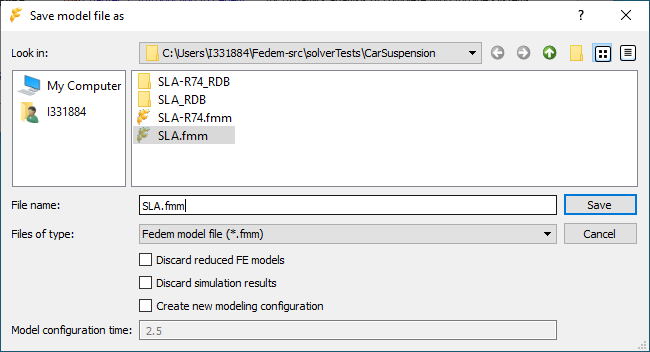
\includegraphics[scale=0.6]{Figures/Dialogs/2-SaveAsUpdated}
\end{figure}

When saving a new model for the first time, you are prompted to give it a name
different from the default name \Untitled, which was assigned when
Fedem was started (see \refSection{starting-fedem}{Starting Fedem}).
If you also have performed some solver tasks before saving the model,
the existing results database will then be moved to the correct location
associated with the new model file name, unless you have toggled on either
Discard simulation results or \textbf{Create new modeling configuration}, see
\protect\hyperlink{saving-a-model-copy-with-results}
                  {\sl"Saving a model copy with results"} below.

\Caution{If you do not save a new model still named \Untitled{}
  before you open another model or Exit Fedem,
  all solver results associated with this model will be deleted, if any.
  This also includes the results of any reductions performed,
  unless FE model repositories were used
  (see \refSection{using-fe-model-repositories}{Using FE model repositories}).}

\SubSubSection{Saving a model copy with results}
              {saving-a-model-copy-with-results}

If the model contains simulation results when you do a \textbf{Save As...},
you will have the options to either \textbf{Discard simulation results} or
\textbf{Create new modeling configuration}, by activating the
associated toggles:

\begin{figure}[H]
  \center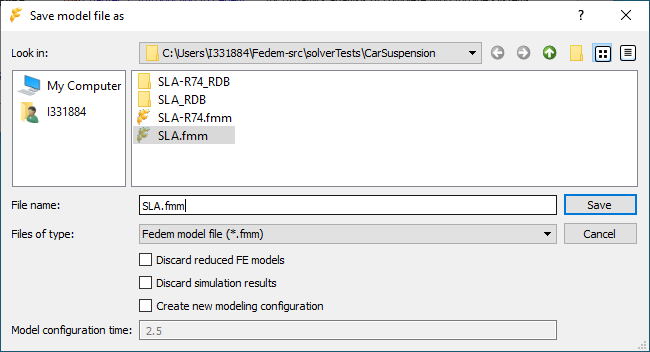
\includegraphics[scale=0.6]{Figures/Dialogs/2-SaveAsUpdated}
\end{figure}

If the latter toggle is activated, you can then specify the simulation
time from which the response state will be used to create a
new modeling configuration, by updating all Triad and Part
positions in the new model.

\subsubsection{Indication on whether a Save is needed}

\begin{wrapfigure}{r}{0.4\textwidth}
  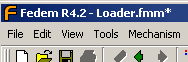
\includegraphics[width=0.4\textwidth]{Figures/2-TitleWithAsterisk}
\end{wrapfigure}

When the current model has been changed compared to the previously saved
version, Fedem will indicate this with an asterisk (*) after
the model file name in the title bar of the main window.
Only if this asterisk is present, you will be asked if you
first want to save the current model when you \textbf{Open} another model,
create a \textbf{New} model, or \textbf{Exit}.


\SubSection{Starting a new model}{starting-a-new-model}

You can at any time during a Fedem session start modeling on a new model.

\IconText{new}{Choose \textbf{New} from the \textbf{File}
  menu, or click the \textbf{New} icon in the tool bar.
  This is equivalent to exiting the current Fedem session and then starting
  a new one (see \refSection{starting-fedem}{Starting Fedem})
  except that the new model now by default will be located in the same directory
  as the current model.}

\Note{If the current model has been modified after the last \textbf{Save},
  you will be asked whether you want to save those changes
  before starting on the new model.}


%%%%%%%%%%%%%%%%%%%%%%%%%%%%%%%%%%%%%%%%%%%%%%%%%%%%%%%%%%%%%%%%%%%%%%%%%%%%%%%%
\Section{Loading and unloading FE-data}{loading-and-unloading-fe-data}

When a model contains several large FE-models, unloading some of the FE-data
from memory can be necessary to in order to reduce the amount of resources used.
This is particularly useful when you want to load contour plots for a
particular part, or to free up resources for the solvers.


\SubSection{FE-data settings}{fe-data-settings}

FE models often tend to be large.
The amount of data needed for visualization and lookup is indeed significant.
In some cases it will be convenient or necessary to unload this data,
to free up RAM.

\IconText{FE-DataSettings}{To control the loading and unloading of FE-data, the
  FE-Data Settings dialog box is used. To open this dialog box (shown below),
  select the \textbf{FE-Data Settings...} command in the \textbf{Tools} menu.}

\begin{wrapfigure}{R}{0.5\textwidth}
  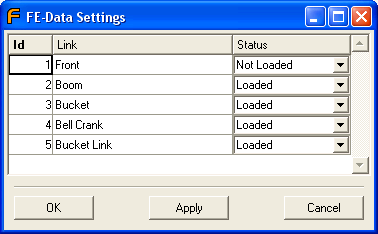
\includegraphics[width=0.5\textwidth]{Figures/Dialogs/2-FE-DataSettings}
\end {wrapfigure}

The status of each FE part is set using the pull-down menu in the {\sl Status}
column. Set the status you want for each part,
and press \textbf{OK} or \textbf{Apply}.
The parts that are not loaded will be shown using the Simplified line shape,
as described in \refSection{item-appearance}{Item Appearance}.

The loading and unloading of FE parts does not affect the simulation.
The solver processes will read the necessary FE-Data from the FE-model files.

\Tip{To change the status of all or several parts quickly, it is convenient to
  use the arrow keys to navigate between the pull-down menus, and the
  \textbf{N} key (Not Loaded) or \textbf{L} key (Loaded) to set the status.}

\Note{Loading unloaded parts can take several minutes if the parts are big.}


\SubSection{Skipping FE-data when opening a model file}{skipping-fe-data-when}

When opening a big model for inspection or simulation, it is sometimes
convenient to override the FE-Data Settings and skip the FE-models
completely. In that way you can open a model containing extremely large
parts in a few seconds, without using any significant amount of memory.

To do this, toggle the {\sl Skip FE-Data} toggle in the Open model file dialog
box when opening a model file, or use the \File{-noFEData} command-line option
together with \File{-f \Variable{modelfilename}} when starting Fedem.

The model will then be loaded with all FE parts unloaded. To load the parts,
open the FE-Data Settings dialog box which now will show the status on the
parts last time you saved your model. If you simply press \textbf{OK} or
\textbf{Apply}, those settings will be applied and the parts that was marked as
{\sl Loaded} will then actually be loaded.


\SubSection{Modeling with unloaded parts}{modeling-with-unloaded-parts}

An unloaded part can generally be used as any other part while modeling,
but there are some restrictions.
When selecting points on the part, the points will not snap to the closest node
because the node information has not been loaded.
The only points on the part that are available for selecting and modeling are
the external nodes represented by the Triads.

Triads can generally not be detached or deleted from unloaded FE parts.
This is done to protect the reduced matrices associated with the part
from being accidentally invalidated.
If you try to to do this, you will instead get an error message instead.
When detaching a Joint from an unloaded FE part,
a Triad will be left on the part where the Joint was attached.


\SubSection{Postprocessing unloaded parts}{postprocessing-unloaded-parts}

Unloaded FE parts will be completely skipped when loading an Animation,
except for the rigid body motion. This makes it possible to focus the
computer resources on the parts of your model that are interesting,
and skip everything else, see also
\refSubSection{disabling-and-enabling}{Disabling and Enabling results}
{result-manipulation}.


%%%%%%%%%%%%%%%%%%%%%%%%%%%%%%%%%%%%%%%%%%%%%%%%%%%%%%%%%%%%%%%%%%%%%%%%%%%%%%%%
\Section{Exporting objects}{exporting-objects}

Fedem can export six types of objects: Parts (FE models), individual
Curves, Graphs, Graph views, the Modeler view and Animations.

\begin{itemize}
\item FE Parts can be exported in Fedem Technology Link (\File{.ftl}) format.
\item Curves and Graphs can be exported in ASCII (\File{.asc}, \File{.txt}),
  nCode DAC (\File{.dac}) or MTS RPC time history (\File{.rsp}, \File{.drv},
  \File{.tim}) format.
\item The Modeler- and Graph views can be exported as binary image files
  in a variety of formats.
\item Animations can be exported as movies
  in \File{.mpeg} and \File{.avi} formats.
\end{itemize}


\SubSection{Exporting a part}{exporting-a-part}

To export an FE Part, complete the following steps:

\noindent
\begin{minipage}{0.65\textwidth}
  \raggedright
  \begin{enumerate}
  \item Right-click the part in the Model Manager {\sl Objects} list to access
    the shortcut menu (partly shown right).
  \item Select \textbf{Export Part...} to open the \newline
    ``Save part as'' dialog box.
  \item Specify a file name and location, \newline
    then click \textbf{Save}.
  \end{enumerate}
\end{minipage}% <--- the % is needed here to kill off spurious spacing
\begin{minipage}{0.35\textwidth}
  \raggedleft
  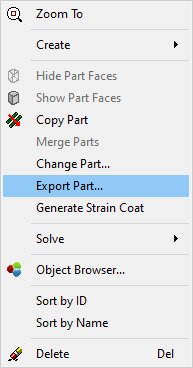
\includegraphics[trim=0 35 0 20,clip,width=\textwidth]{Figures/2-ExportPart}
\end{minipage}


\SubSection{Exporting curves and graphs}{exporting-curves-and-graphs-2}

To export curves, complete the following steps:

\noindent
\begin{minipage}{0.5\textwidth}
  \raggedright
  \begin{enumerate}
  \item Select one or more Curves in the Model Manager {\sl Results} list,
    and right-click your mouse to access the shortcut menu (shown right).
  \item Select \textbf{Export Curves...} to open the dialog box labeled either
    ``Save curve as'' or ``Save curves to directory''.
  \item Depending on your selection, you will be prompted for either a
    file name or a directory.
    If you select multiple curves, the curve files will be named automatically,
    \newline but you have to select what file format you want to export to.
  \end{enumerate}
\end{minipage}% <--- the % is needed here to kill off spurious spacing
\begin{minipage}{0.5\textwidth}
  \raggedleft
  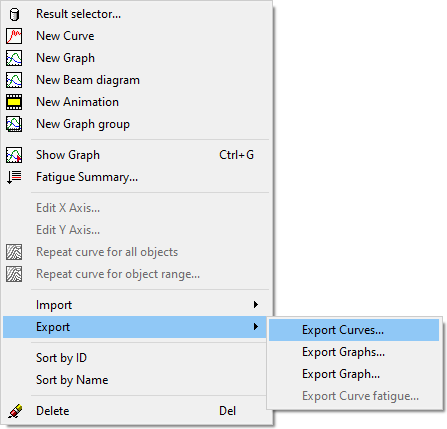
\includegraphics[width=0.95\textwidth]{Figures/2-ExportCurves}
\end{minipage}

To export one or more graphs, complete the following steps:

\begin{enumerate}
\item Select one or more graphs or curves in the Model Manager {\sl Results}
  list and right-click your mouse to access the shortcut menu.
\item Select \textbf{Export} and then \textbf{Export Graphs...} to open the
  dialog box labeled either ``Save graph as'' or ``Save graph to directory''.
\item As when exporting curves, you will be prompted for either a file name
  or a directory depending on your selection. The graph files will be given
  names automatically if you have selected multiple graphs.
\end{enumerate}

For more detailed information on how to export and import curves and
graphs, see \refSection{export-of-curve-data}{Export of Curve Data}
and \refSection{importing-curves-and-graphs}{Importing Curves and Graphs},
respectively.


\SubSection{Exporting the 3D modeler view}{exporting-the-3d-modeler-view}

\noindent
\begin{minipage}{0.41\textwidth}
  \setlength{\parskip}{1mm}
  \raggedright
  To export this view, make it active, then select \textbf{Export} and then
  \textbf{Export View...} from the \textbf{File} menu.

  When exporting the {\sl Modeler} view, you may choose between the following
  image formats:

  \begin{itemize}
  \item\File{.bmp}
  \item\File{.jpeg}
  \item\File{.png}
  \item\File{.rgb}
  \item\File{.iv} \small(3D inventor snapshot)
  \end{itemize}
\end{minipage}% <--- the % is needed here to kill off spurious spacing
\begin{minipage}{0.59\textwidth}
  \raggedleft
  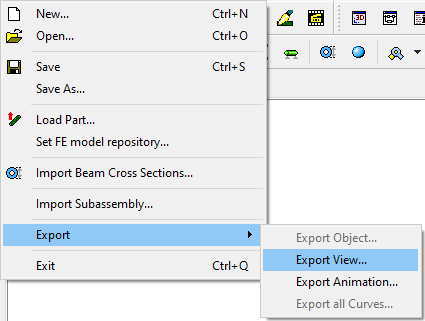
\includegraphics[width=0.95\textwidth]{Figures/2-ExportView}
\end{minipage}

\vskip5mm
The different file formats have different quality.
The format \File{.jpeg} is widely recognized.
The compression reduces the quality somewhat, but the files are small.
The formats \File{.png} and \File{.bmp} have better quality.
We recommend using the \File{.png} format for high quality images.

The \File{.iv} format enables dynamic 3D-viewing of your models using
an external viewer. Viewers are available for several platforms.

Stills of animations, e.g., contour plots, can also be exported.
Simply pause your animation where you want the picture or 3D-snapshot taken,
then export the {\sl Modeler} view.


\SubSection{Exporting graph views}{exporting-graph-views}

To export a {\sl Graph} view, follow the steps described in the section above.
Here you may choose between these image formats:

\begin{itemize}
\item\File{.bmp}
\item\File{.jpeg}
\item\File{.png}
\end{itemize}


\SubSection{Exporting animations}{exporting-animations-intro}

\begin{wrapfigure}{R}{0.5\textwidth}
  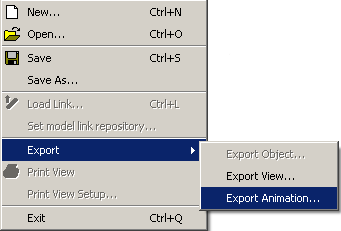
\includegraphics[width=0.5\textwidth]{Figures/2-ExportAnim-sec-2-8-2}
\end {wrapfigure}

Animations can be exported using the \File{.mpeg} (mpeg-1 or mpeg-2) and
\File{.avi} (Windows only) formats. The exported animation may be viewed
in any standard video player, e.g., Windows Media Player or Elecard MPEG
Player (www.elecard.com).

After loading the animation, select \textbf{Export} and then
\textbf{Export Animation...} from the \textbf{File} menu to open a dialog box
where you can select location, file name and format of your exported animation.
See \refSection{exporting-animations}{Exporting animations} for details.

\clearpage


%%%%%%%%%%%%%%%%%%%%%%%%%%%%%%%%%%%%%%%%%%%%%%%%%%%%%%%%%%%%%%%%%%%%%%%%%%%%%%%%
\Section{Customizing Fedem using Plug-Ins}{customizing-fedem-using-plug-ins}

On Windows, plug-ins are provided as DLL-files in the \File{plugins} subfolder
of the installation folder of the Fedem software. Once a plug-in DLL has been
placed in the \File{plugins} folder, it will show up in the Plug-Ins dialog box
in Fedem (see below), which is available from \textbf{Tools} menu.
Here you can tick which plug-ins to use.

\begin{figure}[!h]
  \center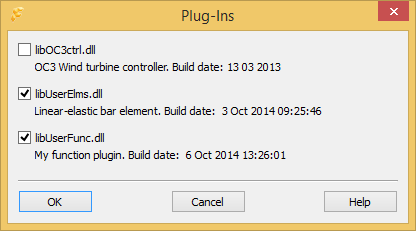
\includegraphics[width=0.6\textwidth]{Figures/Dialogs/2-Plugins}
\end{figure}

Fedem currently provides plug-in interfaces of two kinds; user-defined functions
and user-defined elements. However, only one plug-in of each kind can be
activated at the same time.


\SubSection{User-defined functions}{user-defined-functions}

Fedem provides a range of built-in mathematical functions that may be
used to describe external loads, prescribed motions, etc., in the model
(see \refSection{functions}{Functions}).
In addition, a plug-in architecture for enabling user-defined functions
is provided.

If you wish to implement your own custom functions, you can create your
own plug-in DLL. In the \File{Templates} subfolder of your Fedem installation,
you will find the source code file \File{userfunc.C}, which can be used as
a template for building your own functions plug-in implemented in C or C++.
Build instructions and other explanations can be found as comments in that file.
The user-defined functions from the DLL library will show up in Fedem similarly
as the internal functions described in \refSection{functions}{Functions}.

A user-defined functions plug-in must contain all of the following methods.
The core functionality of the plug-in lies in invoking the method
\protect\hyperlink{ufgetvalue}{\bf ufGetValue}.
You are free to implement the body of this method as you like,
utilizing any other methods and libraries you have available.
This allows for very flexible and powerful additions to the Fedem software,
and can be used to create black-box control systems, or for invoking 3rd-party
calculation engines.

\subsubsection{bool ufGetSignature (int nchar, char* sign)}

This method returns (through the {\sl sign} argument) the name orsignature
of the plug-in library, as it is shown in the Plug-Ins dialog box (see above).

\subsubsection{int ufGetFuncs (int maxUF, int* funcId)}

This method returns (through the {\sl funcId} argument) a list of unique IDs
for each of the user-defined functions in the library.
It can be any integer value, and is used for internal book-keeping only.
The method returns the number of user-defined functions in the library.

\subsubsection{int ufGetFuncName (int id, int nchar, char* name)}

\begin{minipage}{0.49\textwidth}
  \raggedright
  This method defines the {\sl name} of the function with the specified {\sl id}.
  This is the function name as it appears in the {\sl Function type} menu
  of the Function Property Editor panel (shown to the right,
  see also \refSection{function-properties}{Function properties}).
  The method returns the number of function arguments.
\end{minipage}% <--- the % is needed here to kill off spurious spacing
\begin{minipage}{0.51\textwidth}
  \raggedleft
  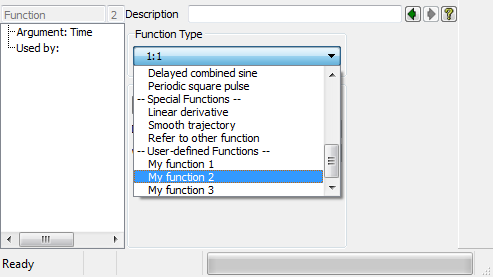
\includegraphics[trim=92 55 90 18,clip,width=0.85\textwidth]{Figures/2-FunctionType}
\end{minipage}

\subsubsection{int ufGetParName (int id, int ipar, int nchar, char* name)}

This method defines the {\sl name} of function parameter number {\sl ipar}
for the function with the specified {\sl id}. This is the parameter name as it
is shown in the parameter list of your function in the Function Property Editor
panel (shown below). The method returns the total number of parameters for the
specified function.

\begin{figure}[!h]
  \center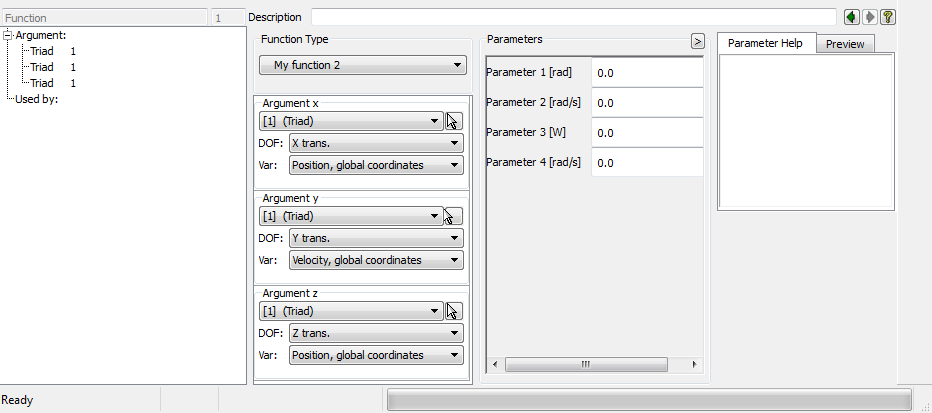
\includegraphics[trim=185 96 20 0,clip,width=0.8\textwidth]{Figures/2-ArgumentsAndParameters}
\end{figure}

\SubSubSection{double ufGetValue (int baseId, int funcId, \\
  const double* par, const double* x, int\& err)}{ufgetvalue}

This method evaluates an instance of the specified function, for a given set of
parameter values ({\sl par}) and argument values ({\sl x}).
This is where you will insert your user-specific code that performs the
function evaluation.

The {\sl baseId} argument is a unique identifier for each function instance,
and is assigned automatically by Fedem. It may be used to identify a certain
instance (if there are more than one) of a given user-defined function within
the plug-in library. The {\sl funcId} argument then has the same value for all
instances of a given function type.

\subsubsection{double ufGetDiff (int baseId, int funcId, int ia, \\
  const double* par, const double* x, int\& err)}

This method evaluates the {\sl ia}$^{th}$ partial derivative of the specified
function for a given set of parameter and argument values.
If you do not require the function derivatives in your application,
you can just leave the body of this method blank and return 0.0.

\Note{You should be aware of the difference between arguments and parameters
  for a user-defined function.
  Arguments are the variables that are linked to simulation results from
  Fedem, such as position, angle, velocity, etc., for a particular part of
  your model. Parameters are additional constant variables that you need
  to evaluate the function. Say, your function is some mathematical
  equation, then the arguments are the equation's variables, while the
  parameters are the equation's various constants.}


\SubSection{User-defined elements}{user-defined-elements}

Fedem provides a plug-in architecture for enabling user-defined finite elements
in a mechanism model.

If you wish to implement your own custom elements, you can create your own
plug-in DLL. In the \File{Templates} subfolder of your Fedem installation,
you will find the source file \File{userelm.C}, which can be used as
a template for building your own finite element plug-in implemented in C or C++.
Build instructions and other explanations can be found as comments in the file.

\clearpage
\begin{wrapfigure}{r}{0.5\textwidth}
  \includegraphics[trim=0 0 0 852,clip,width=0.5\textwidth]{Figures/2-MechanismMenu}
\end{wrapfigure}

When a plug-in DLL with user-defined elements is activated, the element
types contained by it will be listed under the
\textbf{User-defined Elements} sub-menu of the \textbf{Mechanism} menu,
as shown to the right. In this example, the DLL contains one element type
named ``Linear-elastic Bar''.

A user-defined elements plug-in must contain all of the following methods.
The core functionality the plug-in lies in the evaluation of the method
\protect\hyperlink{ueupdate}{\bf ueUpdate}.
You are free to implement the body of this method as you like, utilizing any
other methods and libraries you have available.
This allows for very flexible and powerful additions to the Fedem Dynamics
Solver, providing sets of black-box nonlinear finite elements.

\subsubsection{bool ueGetSignature (int nchar, char* sign)}

This method returns (through the {\sl sign} argument) the name or signature
of the plug-in library, as it is shown in the Plug-Ins dialog box.

\subsubsection{int ueGetElements (int maxUE, int* eType)}

This method returns (through the {\sl eType} argument) a list of unique
IDs for each of the user-defined element types in the library. The IDs
can be any integer value, and is used for internal book-keeping only.
The method returns the number of user-defined element types in the library.

\subsubsection{int ueGetTypeName (int eType, int nchar, char* name)}

This method defines the {\sl name} of the element type with the specified
{\sl eType}. This is the element type name as it appears in the
\textbf{User-defined Elements} sub-menu of the \textbf{Mechanism} menu
(as shown above). The return value is the number of nodes in the specified
element type.

\subsubsection{int ueInit (int eId, int eType, int nenod, int nedof, \\
  const double* X0, const double* T0, int* iwork, double* rwork)}

This method initializes a given user-defined element, and is invoked twice by
the Dynamics Solver for each element instance (identified through the {\sl eId}
and {\sl eType} arguments), before the time integration loop is started.
The arguments of this method have the following interpretation:

\begin{enumerate}
\item{\sl eId} --
  unique ID identifying this element instance (the base ID)
\item{\sl eType} --
  unique ID identifying the element type
\item{\sl nenod} --
  number of element nodes
\item{\sl nedof} --
  number of element degrees of freedom
\item{\sl X0} --
  global nodal coordinates of the element (initial configuration)
\item{\sl T0} --
  global nodal orientations of the element (initial configuration)
\item{\sl iwork} --
  integer work area for this element
\item{\sl rwork} --
  real (double precision) work area for this element
\end{enumerate}

In the first call, the arguments {\sl X0}, {\sl T0} and {\sl rwork} must all be
NULL pointers, and the method then only calculates the required size of the work
areas {\sl iwork} and {\sl rwork} of that particular element.
These size parameters are stored in {\sl iwork}{[}0{]} and {\sl iwork}{[}1{]},
respectively. The work areas are then allocated by the calling program and the
method is called the second time, performing all calculations that are needed
to be done only once for each element instance.
The results of these calculations are stored in the work arrays {\sl iwork} and
{\sl rwork} for later reference by \protect\hyperlink{ueupdate}{\bf ueUpdate}.

The method returns zero on successful exit, and a negative value if any
exception occurs. In the latter case the program execution is aborted.

\SubSubSection{int ueUpdate (int eId, int eType, int nenod, int nedof, \\
  const double* Xn, const double* Tn, \\
  const double* Vn, const double* An, \\
  int* iwork, double* rwork, double* eKt, double* eC, double* eM, \\
  double* eFs, double* eFd, double* eFi, double* eQ, \\
  double t, double dt, int istep, int iter)}{ueupdate}

This method is invoked by the Dynamics Solver, once for each element instance
within the nonlinear iteration loop. It evaluates the updated tangent matrices
and associated right-hand-side force vectors for the specified element.
The body of this method is where you will insert your user-specific code
describing the non-linear finite element behavior.

The arguments no. 5 through 17 ({\sl Xn}, {\sl Tn}, ..., {\sl eQ})
are all C-pointers to arrays which are allocated by the calling program.
The length of these arrays depends on the number of nodal points connected
to the element, and it is the responsibility of the programmer making the DLL
to ensure that access outside the array bounds does not occur.
The interpretation of all the 21 arguments of this method are as follows:

\begin{enumerate}
\item{\sl eId} --
  unique ID identifying this element instance (the base ID)
\item{\sl eType} --
  unique ID identifying the element type
\item{\sl nenod} --
  number of element nodes
\item{\sl nedof} --
  number of element degrees of freedom
\item{\sl Xn} --
  global nodal coordinates of the element (current configuration)
\item{\sl Tn} --
  global nodal orientations of the element (current configuration)
\item{\sl Vn} --
  global nodal velocities of the element (current configuration)
\item{\sl An} --
  global nodal accelerations of the element (current configuration)
\item{\sl iwork} --
  integer work area for this element
\item{\sl rwork} --
  real (double precision) work area for this element
\item{\sl eKt} --
  element tangent stiffness matrix
\item{\sl eC} --
  element damping matrix
\item{\sl eM} --
  element mass matrix
\item{\sl eFs} --
  internal elastic forces of the element
\item{\sl eFd} --
  internal damping forces of the element
\item{\sl eFi} --
  internal inertia forces of the element
\item{\sl eQ} --
  external forces acting on the element
\item{\sl t} --
  current time
\item{\sl dt} --
  time step size
\item{\sl istep} --
  time step number
\item{\sl iter} --
  nonlinear iteration number
\end{enumerate}

The method returns zero on successful exit, and a negative value if any
exception occurs. In the latter case the program execution is aborted.

\subsubsection{Creating user-defined elements}

When creating user-defined elements in a Fedem model, they have to be created
from a set of already created Triads, in a similar fashion as when creating
Beams and Generic Parts:

\begin{enumerate}
\item Create Triads where you want to locate the nodes of the elements.
\item Select the Triads representing the nodes of the element(s), using the
  multi-select features of Fedem (see
  \refSection{model-manager}{Model Manager} and \refSection{select}{Select}).
\item Select the appropriate item from the \textbf{User-defined Elements}
  sub-meny of the \textbf{Mechanism} menu, that represent the type of element
  you want to create.
\end{enumerate}

\clearpage
A set of user-defined elements of the specified type is then created.
The number of elements created is equal to $(n_T-n_{en}+1)$ where $n_T$ is the
number of selected Triads, and $n_{en}$ is the number of nodes per element,
and two elements will then always have $(n_{en}-1)$ nodes in common.
This can be utilized to create strings of two-noded user-defined elements.

\Caution{Pay attention to the order in which you select the Triads to be used,
  as it will reflect the internal nodal ordering of the created element.
  For elements with three or more nodes, the internal ordering is often of
  importance to get a proper solution.}


%%%%%%%%%%%%%%%%%%%%%%%%%%%%%%%%%%%%%%%%%%%%%%%%%%%%%%%%%%%%%%%%%%%%%%%%%%%%%%%%
\Section{Customizing Fedem using Addons}{customizing-fedem-using-addons}

On the Windows platform (Windows 7 and later), Fedem offers the possibility to
extend the modelling and post-processing environment through the use of Addons.

\noindent
\begin{minipage}{0.55\textwidth}
  \raggedright
  The Addons are separate executables that may be launched from the
  \textbf{Addons} menu in Fedem (as shown to the right).
  Each menu item here corresponds to an EXE file in the \File{Addons} subfolder
  of the installation folder of the Fedem software. If that folder is empty or
  does not exist, the \textbf{Addons} menu is absent.
\end{minipage}% <--- the % is needed here to kill off spurious spacing
\begin{minipage}{0.45\textwidth}
  \raggedleft
  \includegraphics[width=0.95\textwidth]{Figures/2-AddonsMenu}
\end{minipage}

The Addons communicate with the main Fedem GUI over a COM API,
which is available for advanced users such that they may program their own
addons for performing certain tasks. This is a powerful means for creating
specialized pre- and post-processors for doing complex modeling tasks.
The Fedem installation does not contain any Addons itself, but some can be
provided as additional packages.
